\documentclass[ITR,BA,english,intermediate, tutorial]{LSR_thesis} 
\graphicspath{{pics/}}
\usepackage{graphicx} 
\usepackage{float}
\usepackage{amsmath}
\usepackage{subfigure} 
\usepackage[colorlinks,linkcolor=blue]{hyperref}
\usepackage{url}
\usepackage[final]{pdfpages}
%% Options:
%% LSR: LSR Template with Prof. Buss as default
%% ITR: ITR Template with Prof. Hirche as default

%% BA: Bachelorarbeit / Bachelor thesis
%% MA: Masterarbeit / Master thesis
%% HS: Hauptseminar / Scientific seminar
%% PP: Projektpraktikum / practical course
%% IP: Ingenieurpraxis
%% FP: Forschungspraxis
%% SeA: Semesterarbeit (MW)

%% english
%% german

%% final
%% intermediate

%% tutorial -> remove flag such that help files and todos are removed

%%% last changes: 11.03.2020 (tim.bruedigam@tum.de)

%------------------------------------------------%
%_________CUSTOMIZE LATEX ONLY IN customize.tex!_% 
%_________ DO NOT MODIFY THE TEMPLATE!___________%
%________________________________________________%
% add customize first so you can access your commands in gloss, or fuse both into one file
%%%%%%%%%%%%%%%%%%%%%%%%%%%%%%%%%%%%%%%%%%%%%%%%%%%%%%%%%%%%%%
% CUSTOMIZING Tex-File for students to be adjusted as needed %
%%%%%%%%%%%%%%%%%%%%%%%%%%%%%%%%%%%%%%%%%%%%%%%%%%%%%%%%%%%%%%
%%%%%%%%%%%%%%%%%%%%%
% CUSTOM PACKAGES	%
%%%%%%%%%%%%%%%%%%%%%
\usepackage{tikz}
\usepackage{pgfplots}

% \usepackage{IEEEtrantools}

%%%%%%%%%%%%%%%%%%%%%
% CUSTOM COMMANDS	%
%%%%%%%%%%%%%%%%%%%%%
% e.g. Math conventions as vectors, Matrices, sets
\renewcommand{\vec}[1]{\mathbf{\MakeLowercase{#1}}}
\newcommand{\Mat}[1]{\mathbf{\MakeUppercase{#1}}}
\newcommand{\set}[1]{\boldsymbol{#1}}

% e.g. use differenc layers in tikz
\pgfdeclarelayer{background}
\pgfdeclarelayer{nodelayer}
\pgfdeclarelayer{edgelayer}
\pgfdeclarelayer{foreground}
\pgfsetlayers{background,edgelayer,nodelayer,main,foreground}
%%%%%%%%%%%%%%%%%%%%%
% HYPHENATIONS 		%
%%%%%%%%%%%%%%%%%%%%%
\hyphenation{Lya-pu-nov}

 % add custom commands etc in this file 
% %%%%%%%%%%%%%%%%%%%%%%%%%%%%%%%%%%%%%%%%%%%%%%%%%%%%%%%%%%%%%%
% NOTE: Using this is optional
% 	Nonetheless, feel free to include this file and adjust the 
% 	examples below as needed
%   
% Questions, feedback and improvements:
%	-> https://git.lsr.ei.tum.de/students/student-templates/issues
% ATTENTION:
% 	- Keep in mind that thif file uses the \vec and \mat commands
% 	 	which are defined in customize.tex!
%	- add glsaddall if you want all of the elements in gloss.aux
%		being printed into your list of acronyms.
% Further reading:
%	https://ctan.org/pkg/glossaries?lang=en
%%%%%%%%%%%%%%%%%%%%%%%%%%%%%%%%%%%%%%%%%%%%%%%%%%%%%%%%%%%%%%

% include packages
\usepackage{setspace}
\usepackage{filecontents}
% for sharelatex, the indexing using xindy:
% 	http://xindy.sourceforge.net/doc/faq-1.html#ss1.2
% is not available, thus the adjustments below ar necessary
%% Adjust Flag for Sharelatex
\newif\ifShareLatex 
%\ShareLatextrue            	% if you work in sharelatex: https://sharelatex.tum.de
\ShareLatexfalse          		% if you work locally

\ifShareLatex
    \usepackage[acronym, style=alttree, shortcuts, toc=true, nomain, nonumberlist]{glossaries}
    \renewcommand{\makeglossaries}{\makenoidxglossaries}
    \renewcommand{\printglossary}{\printnoidxglossary}
\else
    \usepackage[acronym,style=alttree, toc=true, shortcuts, xindy, nomain, nonumberlist]{glossaries}
    \RequirePackage[xindy]{imakeidx}
\fi

%%%%%%%%%%%%%%%%%%%%%%%%%%%%%%%%%%
% DEFINE HEADINGS AND CATEGORIES %
%%%%%%%%%%%%%%%%%%%%%%%%%%%%%%%%%%
% preferable use a command, to adjust the Capitalization 
% for the header section of fancyhdr automatically
\newcommand{\Symbols}{List of Symbols}
\newcommand{\Notation}{Notation}
\newglossary{symbols}{sym}{sbl}{\Symbols}
\newglossary{notation}{not}{nt}{\Notation}
% set width of first row
\glssetwidest{THISWIDE}     % adjust length as needed

%%%%%%%%%%%%%%%%%%%%%%%%%%%%%
% DEFINE ACRONYMS/GLOSSARY	%
%%%%%%%%%%%%%%%%%%%%%%%%%%%%%
\makeglossaries % don't remove this
\begin{filecontents}{gloss.aux}
	%===========%
	% ACRONYMS	%
	%===========%
	\newacronym{MPC}{MPC}{model-predictive control}
	\newacronym{BIBO}{BIBO}{bounded-input bounded-output}
	\newacronym{HRC}{HRC}{Human-Robot Collaboration}
	%============%
	% SYMBOLS	%
	%===========%
	\newglossaryentry{control}{type=symbols,
		sort={control},
		name={\ensuremath{\vec{u}}},
		description={control input vector}
	}
    \newglossaryentry{uk}{type=symbols,
		sort={control},
		name={\ensuremath{\vec{u}_k}},
		description={control input vector with time step}
	}
    \newglossaryentry{xk}{type=symbols,
		sort={state},
		name={\ensuremath{\vec{x}_k}},
		description={state vector with time step}
	}
	%============%
	% NOTATION	%
	%===========%
	\newglossaryentry{vector}{type=notation,
		sort={vector},
		name={\ensuremath{\vec{x}_n}},
		description={$n$-dimensional vector named $x$}
	}	
	\newglossaryentry{matrix}{type=notation,
		sort={vector-matrix},
		name={\ensuremath{\Mat{x}_{m\times n}}},
		plural={matrices},
		user1={Mat},
		description={\ensuremath{m\times n} dimensional Matrix  named \ensuremath{X}}
	}	
\end{filecontents}
\loadglsentries{gloss.aux}

%%%% Add GLOSSARIES at end of thesis
\newcommand{\AddMyGloss}{
	\renewcommand{\glsglossarymark}[1]{}
   	\printglossary[type=acronym]
	\markboth{\MakeUppercase{acronyms}}{\MakeUppercase{acronyms}}
  	\ifdefined\Symbols
		\printglossary[type=symbols, nogroupskip]
		\markboth{\MakeUppercase{\Symbols}}{\MakeUppercase{\Symbols}}
	\fi
	\ifdefined\Notation
		\printglossary[type=notation, nogroupskip]
		\markboth{\MakeUppercase{\Notation}}{\MakeUppercase{\Notation}}
	\fi
}

		% add your glossary in this file 


%_______Start_Document______________________________________
\begin{document}
%%%%%%%%%%%%%%%%%%%%%%%%%%%%%%%%%%%%%%%%%%%%%%%%%%%%%%%%%%%%%%%
%%%%%%%%%%%%%%%%%%% title page %%%%%%%%%%%%%%%%%%%%%%%%%%%%%%%%
%%%%%%%%%%%%%%%%%%%%%%%%%%%%%%%%%%%%%%%%%%%%%%%%%%%%%%%%%%%%%%%
%% for an english theis. The title:
\title{Quantifying Information Loss Resulting from Degradation of IMU Sensor Resolution in PD Symptom Classification}
%% Für deutsche Arbeiten: Deutscher Titel:
%\title{Die Antwort auf Alles und Mehr - Ein Trauerspiel in 4 Akten}
% and English translation (optional)
\titletranslation{
%Die Verwendung eines Deutschen Untertitels obliegt der Verantwortung der entsprechenden Betreuer
}
% data about YOU!:
\student{Shuyang Tian} 			%% your name
\studtitle{Bachelor of Science} 			%% Bachelor of Arts, Dr.~phil, etc.
\street{Helene-Mayer-Ring 12}			%% your address
\city{80809 Munich}								%		"
\phone{049- 15224376828}			%% your telephone-no.

%% if more students are involved (e.g. PP) 
%--the following parted is not tested ---
% please report bugs to v.gabler@tum.de 
%\studenttwo{Zweiter Student}
%\studtitletwo{} 
%\studentthree{} 
%\studtitlethree{} 
%\studentfour{} 
%\studtitlefour{} 
%-----------------------------------------
\supervisor{Satoshi Endo,Das, Neha,
}			%% your supervisor
\finalrep{11.03.2021}						%% final presentation / date

\maketitle
%%%%%%%%%%%%%%%%%%%%%%%%%%%%%%%%%%%%%%%%%%%%%%%%%%%%%%%%%%%%%%%
%%%%%%%%%%%%%%%%%%%%%%%%%%%%%%%%%%%%%%%%%%%%%%%%%%%%%%%%%%%%%%%

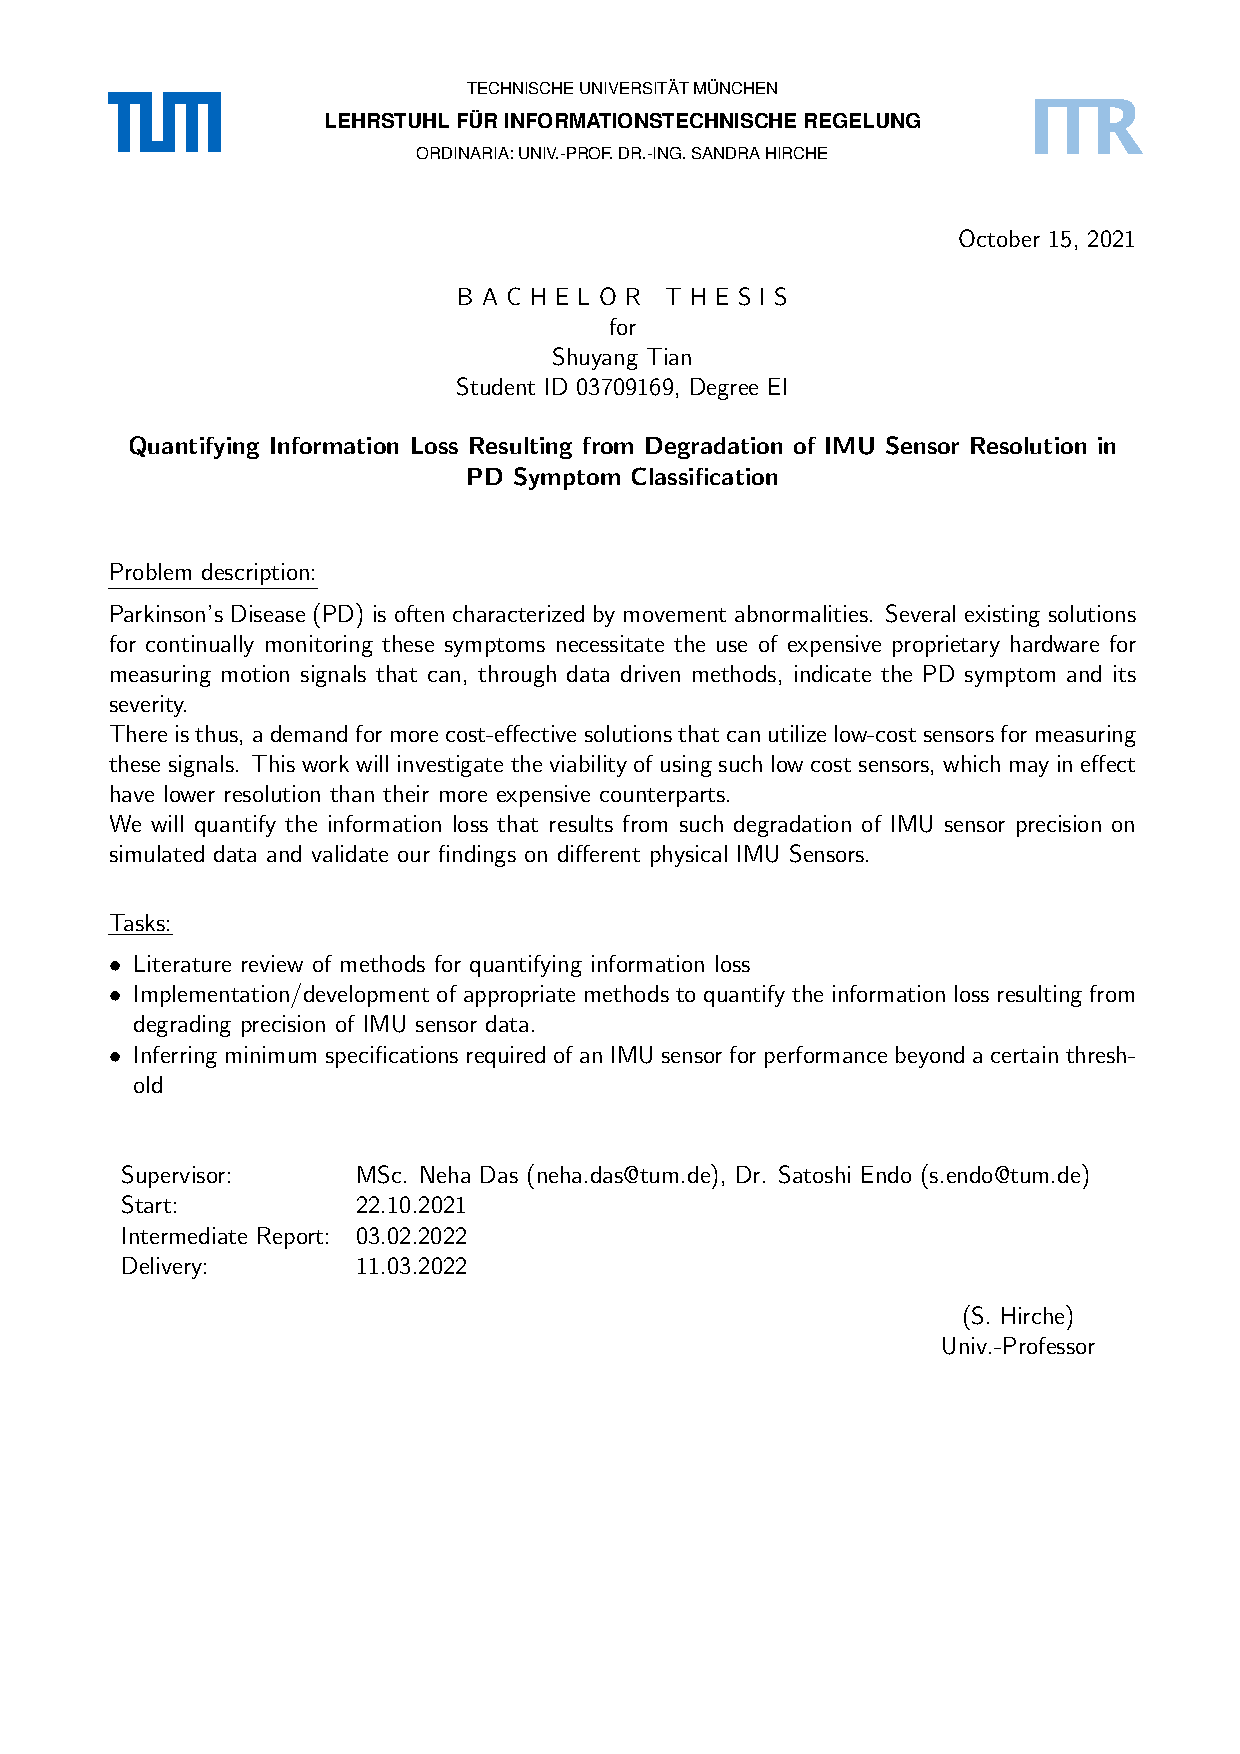
\includepdf{BA_Thesis_Info_Loss_141021.pdf}

\newpage

%%%%%%%%%%%%%%%%%%%%%%%%%%%%%%%%%%%%%%%%%%%%%%%%%%%%%%%%%%%%%%%
%%%%%%%%%%%%%%%%%%%%% abstract %%%%%%%%%%%%%%%%%%%%%%%%%%%%%%%%
%%%%%%%%%%%%%%%%%%%%%%%%%%%%%%%%%%%%%%%%%%%%%%%%%%%%%%%%%%%%%%%
\topmargin5mm
\textheight220mm
\pagenumbering{arabic}
\phantom{u}
\begin{abstract}
  Abnormal movements are often characteristic of Parkinson's disease (PD), and to monitor these movements, IMU sensors can be used to measure the movement signal. Due to the high cost of high-resolution sensors, we will investigate the feasibility of using low-cost sensors, i.e., low resolution. This work will quantify the loss of information to the activity dataset due to the reduced resolution of the IMU sensors. After acquiring the IMU dataset at the original sampling rate, it will be resampled using a different sampling rate to simulate the dataset later collected by the low-resolution IMU sensor. We will then extrapolate the minimum requirements for the IMU sensor within a certain threshold. For this work, we first classify the inertial measurement unit (IMU) data and ratings of Parkinson's symptoms by the k-Nearest Neighbor (KNN) algorithm. Then, by calculating the information loss between different sampling frequencies, we can observe the change in information loss that accompanies the decrease in sampling frequency to derive a threshold value.
%\begin{center}	
%\normalsize \textbf{Zusammenfassung}\\
%\end{center}
%Hier die deutschsprachige Zusammenfassung. 
%\optional{Talk to your supervisor if this is needed and/or wanted before starting with your thesis}
\end{abstract}
\newpage

%%%%%%%%%%%%%%%%%%%%% Widmung %%%%%%%%%%%%%%%%%%%%%%%%%%%%%%%%%
\phantom{u}
\phantom{1}\vspace{6cm}
\begin{center}
%Hier die Widmung oder leer lassen
\end{center}

\pagestyle{fancy}

%%%%%%%%%%%%%%%%%%%Inhaltsverzeichnis%%%%%%%%%%%%%%%%%%%%%%%%%%
\tableofcontents 

%%%%%%%%%%%%%%%%%%%%%%%%%%%%%%%
% ACTUAL CONTENT OF YOUR WORK %
%%%%%%%%%%%%%%%%%%%%%%%%%%%%%%%
%%%%%%%%%%%% Kapitel - externe Dateien zur Ordnung%%%%%%%%%%%%%
\ifLSRITRtutorial
	




\fi
%_________Einleitung__________________________________
\chapter{Introduction}
\label{sec:introduction}

Parkinson's disease (PD) is a chronic neurodegenerative disease affecting the central nervous system, mainly the nervous motor system.\cite{NIND} Its symptoms usually appear slowly over time, with the most prominent early symptoms being tremors, limb stiffness, reduced motor function, and abnormal gait. There may also be cognitive and behavioral problems; dementia is quite common in patients with severe disease. Major depressive disorder and anxiety disorders also occur in more than a third of cases. Other symptoms accompanying the disease include perception, sleep, and mood problems. The main motor symptoms associated with Parkinson's disease are collectively known as Parkinson's syndrome. Parkinson's disease has four main motor symptoms: tremor, bradykinesia, dyskinesia, and postural instability. \\ \cite{NIND,SAMII20041783}

Tremor is the most apparent and well-known symptom, it occurs most often in the hands or arms, but the trunk or head may also be affected. People with Parkinson's disease do not tremble at the beginning of the disease, but most patients gradually develop this symptom as the disease progresses. In Germany, at least one in every hundred people suffers from primary tremor, i.e., tremor without an identifiable underlying neurological disorder.\cite{Klinik} A tremor in Parkinson's disease is most pronounced when the limb is at rest but disappears during sleep or when the limb is consciously moved. Tremor affects more of the distal extremities, usually appearing initially in one hand or foot at the onset but then spreading to both hands and feet. \\

Bradykinesia is another feature of Parkinson's disease, where the patient's movements are slowed down and affect the entire process from movement initiation to execution. The patient cannot make continuous movements or perform different movements simultaneously. \cite{SAMII20041783} Bradykinesia, a form of hypokinesia, emphasizes the slow movement of motor execution and is a common symptom in the early stages of Parkinson's disease. The effects of bradykinesia vary according to the type of movement and the patient's physical and mental state—the patient's mobility and emotional state influence the degree of impact. In general, patients with Parkinson's disease can improve their symptoms of bradykinesia with treatment.\\

Dyskinesia is caused by increased muscle tone and sustained muscle contraction, resulting in difficulty moving the limbs. Limb stiffness may also be associated with arthralgia, which is often present in the early stages of the disease. In the early stages of Parkinson's disease, limb stiffness is often asymmetrical. It tends to develop in the neck and shoulders, then spreads to the face and extremities, and eventually to the whole body as the disease progresses, causing a gradual loss of movement.\cite{jankovic2008parkinson}  Bradykinesia, dyskinesia, tremor will discuss these three types for our classification of Parkinson's patients' symptoms. 
\\ \hspace*{\fill} \\
Parkinson's disease may also have other symptoms, as shown in figure 1.1. The patient may have little or no facial expressions in the early stages and may not swing their arms when walking. However, as the disease progresses, there will probably be changes in speech and writing.



\begin{figure}[htbp]
\centering
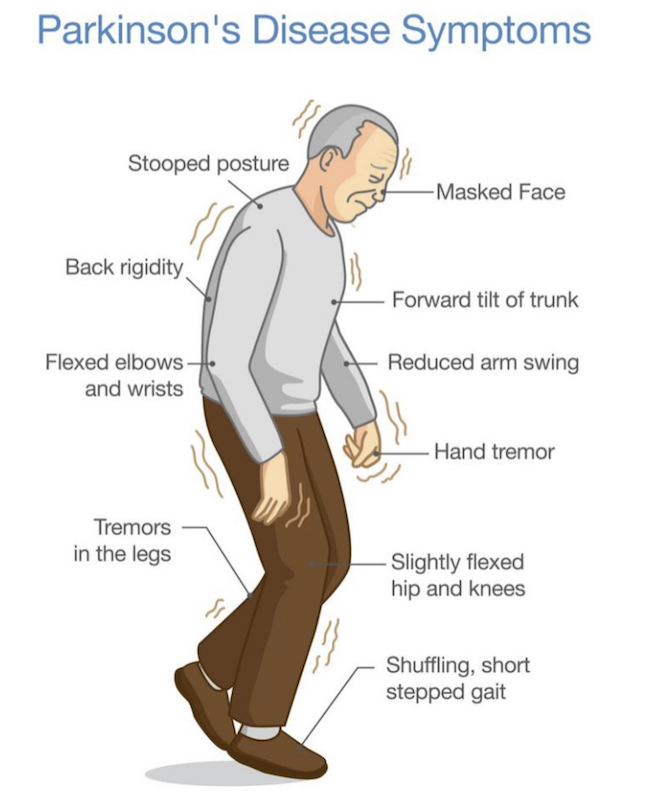
\includegraphics[width=8cm ]{slides-tex/pics/Parkinson's Disease Symptoms.png}
\caption{Parkinson's Disease Symptoms \cite{Symptoms}}
\end{figure}


\\ \hspace*{\fill} \\
Today, IMU sensors are widely used to study Parkinson's motor disease. Chapter 2 clearly describes how IMU sensors work. IMU sensors can collect motion data from the hands or feet of Parkinson's patients, and this motion data can help us analyze Parkinson's disease. However, there are many IMU sensors on the market at different prices, such as aerospace-grade sensors, which are sold at high prices and are used in military aerospace and other fields. In contrast, commercial IMU sensors are relatively inexpensive. Differences in IMU accuracy also determine price differences. Our work quantifies the loss of information when the resolution of IMU sensors is reduced. We resample the dataset collected by the original IMU sensor to create a simulated dataset collected by a low-resolution IMU sensor. After quantifying the information loss, we can infer that the IMU sensor works well at reduced resolution. First, we chose a 5-second Parkinson's time as the test dataset. We want to calculate the information loss by obtaining the predicted classification probability after classification using KNN. It is challenging to handle a super large amount of data. So we made a new step based on the mutual information between IMU data (acceleration data) and symptom score data. We want to calculate the information loss by obtaining the predicted classification probability after classification using KNN. Therefore, we obtained the information loss by simplifying the mutual information formula, as explained in Chapter 3. Chapter 5 specifies the definition of the dataset and variables we use. Chapters 6 and 7 discuss the procedures and methods for calculating the information loss based on KNN classification.

\\ \hspace*{\fill} \\












%____________________________________________________
\chapter{Technical equipment}

\section{Inertial measurement unit}
Inertial measurement unit (IMU) data, an inertial measurement unit (IMU), usually refers to a combined unit consisting of three accelerometers and three gyroscopes mounted on mutually perpendicular measurement axes.\cite{iosa2016wearable} Inertial sensors including accelerometers (or accelerometer sensors) and angular velocity sensors (gyros) and their single, dual, and triaxial combinations IMU (Inertial Measurement Unit), AHRS (Attitude Reference System including magnetic sensors). IMU sensors are used in everyday life, smartphones, smartwatches, and commercial drones, among other electronic products. Commercially available off-the-shelf IMU sensors are small, lightweight, wireless devices that IMU sensors can quickly fix to a body part without interfering with motion. Depending on their application, they are typically embedded in Bluetooth/wireless transmitters or SD cards for real-time data streaming or onboard long-term data recording, respectively.
\begin{figure}[htbp]
\centering
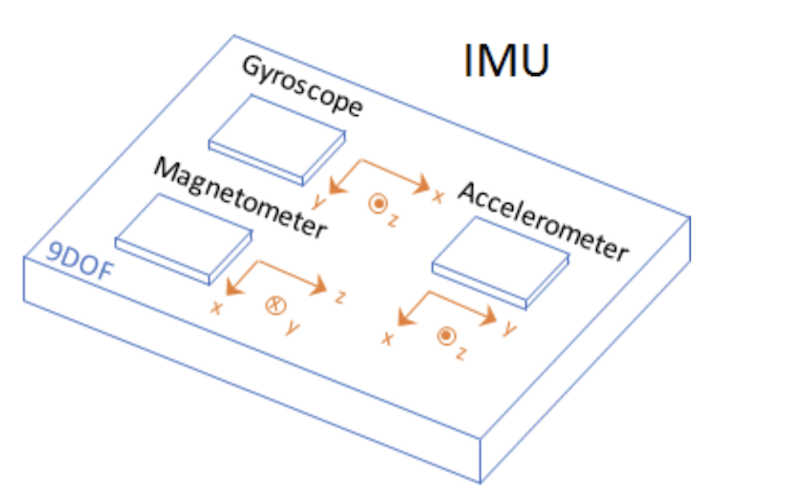
\includegraphics[width=9cm]{report/pics/IMU Sensor .png}
\caption{IMU Sensors' internal structure includes an accelerometer, Magnetometer, and gyroscope.\cite{IMU} }
\end{figure}\\
\section{Working Principle}
 An IMU sensor unit working can be done by using one or more accelerometers to detect linear acceleration and similarly by using gyroscopes to detect rotation rates and magnetometers. \cite{hazry2009study}
 
 
 \section{IMU sensors in our work}
Nowadays, wearable IMU sensors are widely used in medical research, and the acceleration data collected by IMU helps to predict and analyze patient data in the future. Wearable IMU sensors will collect daily data from Parkinson's patients in our present work. We will collect acceleration and angular acceleration from the wrists, ankles, and other body parts of people with Parkinson's disease. We use the MJFF Levodopa wearable sensor dataset \cite{MJFF}, and the Fox Foundation collects wearable sensor data from patients with Parkinson's disease (PD). Subjects were recruited from two clinical sites and monitored while performing a range of routine activities in the clinic and daily activities at home. In Chapter 5, we describe the data collection information in detail.\\

\begin{figure}[htbp]
\centering
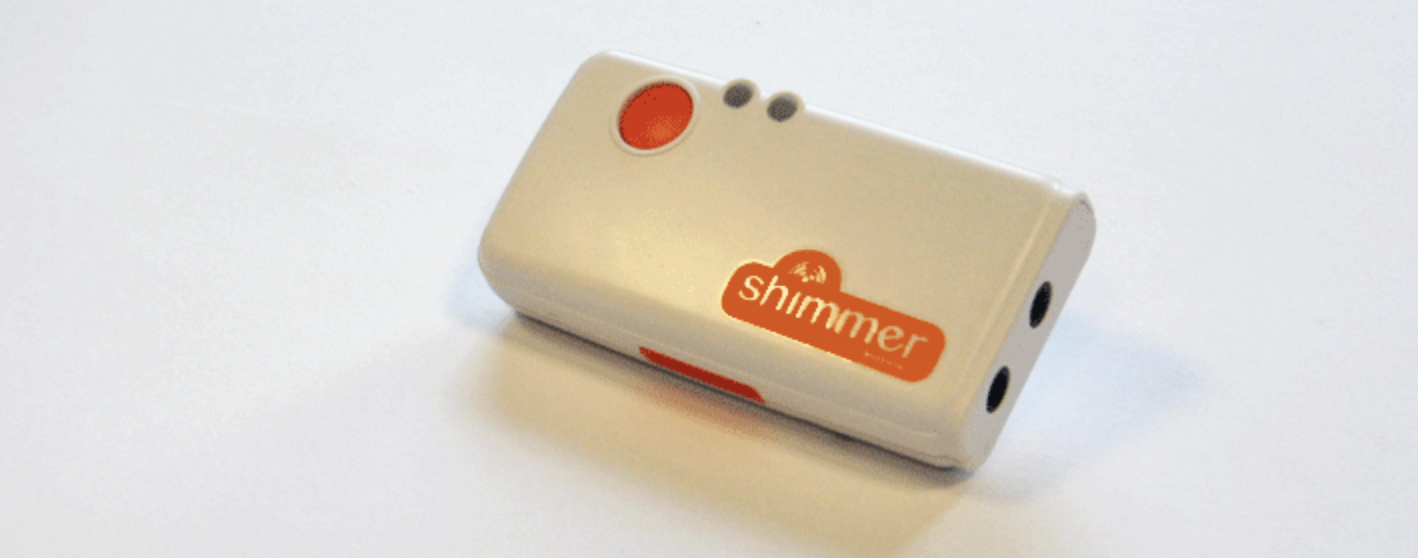
\includegraphics[width=9cm]{report/pics/Shimmer Sensor.png}
\caption{Shimmer3 offers the best data quality with integrated 9DoF inertial sensing via accel, gyro, mag, and pressure sensor, each with selectable range.} \cite{ShimmerSensor}
\end{figure}
The Shimmer sensor is used in medical, neuroscience, and clinical research and is a highly accurate IMU sensor. The Shimmer IMU comes with integrated 9 DoF + altimeter inertial sensing via accelerometer, gyroscope, and magnetometer, each with a selectable range.\cite{ShimmerSensor} But the shimmer sensor is not cheap. Just one Shimmer sensor needs to spend 598 euros. The truth is that IMU sensors are ubiquitous in our lives, such as cell phones and smartwatches. So it is better value for money to wear a watch and a cell phone than to wear a professional IMU sensor.





\chapter{Theoretical background}

\section{Entropy}

The entropy of a random variable is a function that describes the ''unpredictability'' of the random variable. In information theory, entropy is the average amount of information contained in each piece of information received, also known as information entropy. \cite{shannon1948mathematical,PATHRIA201139}
\\ \hspace*{\fill} \\
 The information entropy formula given by Shannon \cite{shannon1948mathematical} , for random variable X, is defined as follows, in bits: \\
\begin{equation}
H(X) = - \sum_{i=1}^{n}p(x_{i}) log(p(x_{i}) )  
\end{equation} 
where $p(x_{i})$ represents the probability of the random variable $x$.
\\ \hspace*{\fill} \\
How much information one has needs to be measured by the amount of information. The amount of information received is related to the specific events that occurred. Therefore, the quantity of information is related to the probability of a random event. The smaller the probability of something happening, the greater the quantity of information generated, for example, an earthquake in one part of the earth; the greater the probability of something happening, the smaller the quantity of information generated, for example, the sun rises in the east every day.
\\ \hspace*{\fill} \\
While the information measure is the information brought about by a specific event that has occurred, the entropy is the expectation of the amount of information that possibly generated before the outcome - considering all possible values of that random variable, i.e., the expectation of the amount of information brought about by all possible events.
\\ \hspace*{\fill} \\
The joint entropy measures the uncertainty associated with a set of variables. The joint entropy of two random $X$ and $Y$ variables is defined as: \cite{cover1999elements}
\begin{equation}
H(X,Y) = - \sum_{x}\sum_{y}p(x,y)\log_{2}{p(x,y)}   
\end{equation} 
 Also, the joint entropy satisfies symmetry, i.e. $H(X,Y) = H(Y,X)$ .\\
 
 The conditional entropy quantifies the amount of information needed to describe the outcome of a random variable Y, given that the value of another random variable X is known. The entropy of Y conditioned on X is defined as:
 

\begin{equation}
\begin{split}
H(Y|X) &= \sum_{x\in \mathcal{X}}p(x)H(Y|X = x) \\
&= -\sum_{x\in \mathcal{X}}p(x)\sum_{y\in \mathcal{Y}}p(x,y)\log_{}{p(y|x)} \\
&= -\sum_{x\in \mathcal{X}}\sum_{y\in \mathcal{Y}}p(x,y)\log_{}{p(y|x)}   \\
&= -\sum_{x\in \mathcal{X},y\in \mathcal{Y}}p(x,y)\log_{}{p(y|x)}  \\ 
&= E_{p(x,y)}\left [ -\log_{2}{p(y|x)}  \right ]  
\end{split}
\end{equation}

The Bayesian rule for conditional entropy is expressed as:
\begin{equation}
H(Y|X) = H(X|Y) - H(X) + H(Y)
\end{equation}

\section{Mutual Information}
Suppose there exists a random variable X , and another random variable Y , then their mutual information is defined as : \cite{cover1999elements}
\begin{equation}
I(X;Y) = \sum_{x,y}p(x,y)\log{\frac{p(x,y)}{p(x)p(y)} }  = H(X) - H(X\mid Y)
\end{equation} 
Similarly, the MI between two continuous random variable X and Y is defined as : 
\begin{equation}
I(X;Y) = \iint_{x,y}p(x,y)\log{\frac{p(x,y)}{p(x)p(y)} } = H(X) - H(X\mid Y) 
\end{equation} 
\\ \hspace*{\fill} \\
,where $p(x,y)$ is the joint probability density and, 
\begin{equation}
p(x) = \int \mathrm{d}yp(x,y) \quad and \quad p(y) = \int \mathrm{d}xp(x,y)
\end{equation} 
are the marginals. \cite{carrara2020estimation}
\\ \hspace*{\fill} \\
In 1948, Shannon defined and analyzed this metric, and later Mutual Information was created by Robert Fano \cite{1057418}. MI also affects the difference between the joint distribution of random variables $(X, Y)$ and the product of the bounded distributions of $X$ and $Y$, as we can find from equations (2.3) and (2.4). MI measures the amount of information obtained about one random variable through observing the other random variable. MI can represent a higher-order relationship among variables.\\
At the same time, mutual information can be equivalently expressed as: \cite{mackay2003information}
\begin{equation}
\begin{split}
I(X;Y) &= H(X) - H(X|Y) \\
&=H(Y) - H(Y|X) \\
&=H(X) + H(Y) - H(X,Y) \\
&=H(X,Y) - H(X|Y) - H(Y|X) \\
\end{split}
\end{equation}
The relationship between mutual information and information entropy is shown in the following figure:
\begin{figure}[htbp]
    \centering
    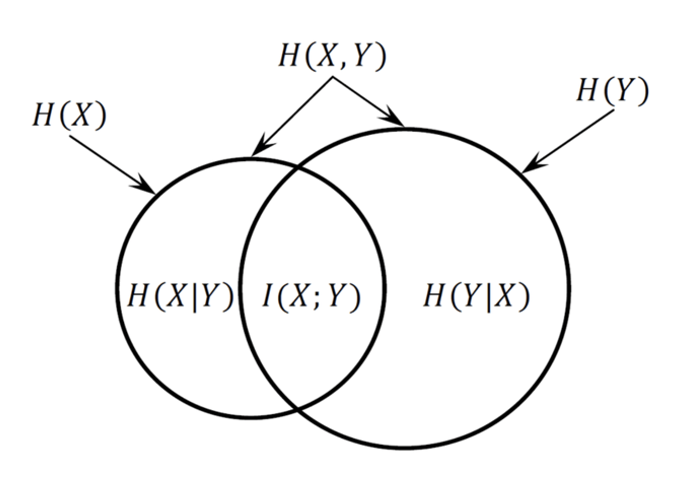
\includegraphics[width=9cm]{report/pics/MI.png}
    \caption{The relationship between mutual information and information entropy}
    \label{fig:my_label}
\end{figure}\\
The figure shows that the two independent variables $X$ and $Y$ are independent when the mutual information $I (X, Y)$ is equal to zero. Also, the mutual information $I (X, Y)$ must be greater than or equal to $I_{min} = 0 $.


\section{Loss of information}
From the theory of mutual information, we know that as $X$ and $Y$ become more correlated, the value of mutual information will become more prominent. A $X$ and $Y$ tend to be independent. The mutual information will become smaller. Therefore, we conjecture that the difference in mutual information will be the amount of information loss concerning information loss. We define information loss as:
\begin{equation}
Loss = I(X;Y) - I(X';Y)
\end{equation}
Under the condition that the mutual information satisfies the symmetry, we take equation (3.8) into (3.9) and get
\begin{equation}
\begin{split}
Loss &= I(X;Y) - I(X';Y)\\
&= I(Y;X) - I(X';Y)\\
&=H(Y) - H(Y|X) - H(Y) + H(Y|X')\\
&=H(Y|X') - H(Y|X)
\end{split}
\end{equation}
\\ \hspace*{\fill} \\
The simplification gives us equation (3.9) which shows that the information loss we calculate equals the difference in conditional entropy for different X and X' relative to Y. The simplified formula avoids the need to calculate other entropy values, thus making it easier for us to work.


\section{Monte Carlo method}
 The Monte Carlo method, also known as the statistical simulation method, is a numerical calculation method guided by statistical probability theory due to the development of science and technology and the invention of electronic computers in the mid-1940s. The Monte Carlo method uses computer-generated samples of a given probability distribution to produce plug-in estimates of specific characteristics of the given distribution. \cite{anderson1986scientific,binder1993monte} \\
\subsection{Monte Carlo approximation}
Suppose X is a random variable with a distribution function $F_{X}(x)$ and suppose that we can generate (through a computer) a sample: \cite{MonteCarlo}
\begin{equation} \nonumber 
\xi _{n} = \left [ x_{1} \dots x_{n}  \right ]  
\end{equation}
of realizations of  n random variables  $X_{1}, ..., X_{n}$ all having distribution function  $F_{X}$. \\

Denote by $F_{n}(x)$ the empirical distribution of the sample $\xi _{n} $ (i.e.,a probability distribution that assigns probability $\frac{1}{n}$ to each one of the values $x_{1}, ..., x_{n}$ .)
Then, the plug-in estimate is a Monte Carlo approximation : 
\begin{equation} \nonumber 
T(F_{n} )  
\end{equation}

\subsection{Monte Carlo integration}
We can approximate an expectation using Monte Carlo integration, which consists of the average of a random sample of observations drawn from the distribution of X to approximate the expectation of the random variable X:  \cite{MonteCarlo}
\begin{equation} \nonumber 
E\left [  X \right ] =\simeq \frac{1}{n}\sum_{i=1}^{n}x_{i}   
\end{equation}
This approximation method is called Monte Carlo integration because the expected value being approximated is in fact an integral:
\begin{equation} \nonumber 
E\left [  X \right ] = \int_{-\infty }^{\infty}x\mathrm{d}F_{X}(x)   
\end{equation}
where $F_{X}(x)$ is the distribution function of $\mathcal{X}$.
Moreover, if  X is a continuous variable, the integral can be written as an ordinary Riemann integral:
\begin{equation} \nonumber 
E\left [ X \right ] = \int_{-\infty }^{\infty } x f_{X}(x)\mathrm{d}x  
\end{equation}
where $f_{X}(x)$ is the probability density function of $\mathcal{X}$.
\chapter{Related Work}

\section{Quantifying information loss}

From Eric Clarkson's \emph{Quantifying the Loss of Information from Binning List-Mode Data} \cite{2020} \\
This paper proposes quantifying the information loss when list pattern data are effectively binned due to analysis operations. In this paper, the authors show that Fisher information loss is actual and use the Fisher information matrix (FIM) to quantify the loss due to binning. Factors affecting information loss are also derived. The list-based model imaging system applies Poisson statistics. It gives the list's conditional distribution probability (PDF) at a fixed exposure time, i.e., $pr(A|\theta)$, where $\theta$ is a p-dimensional parameter vector describing the imaged object. In addition, the authors define the FIM of the list pattern data about $theta$ and the binning FIM. The authors discuss the relationship between the two FIMs by replacing the parameter $\theta$ with the spatial coordinate function $f(r)$, and finally by weighting the Hilbertspacenorm, after which the difference between the two FIMs is the information loss quantified in the article. The paper demonstrates a loss of Fisher information in any estimation task when the data in list mode is binned. The method is also applicable when the estimation problem is an object reconstruction problem, where a finite-dimensional parameter vector is replaced by a function in an infinite Hilbert space. This method gives us the proposal to calculate the loss by computing the Fisher information matrix. However, replacing the parameters as a function in Hilbert space is not easy. Moreover, the method is proposed under Poisson distribution. However, for our IMU data and Parkinson's disease score data, we do not know which distribution probability the data belongs to, so if we use this method, we need to discuss the distribution of our data first.

\\ \hspace*{\fill} \\
From Harikrishnan, K.P. and Misra, R. and Ambika, G's \emph{Quantifying information loss on chaotic attractors through recurrence networks} \cite{2019} \\
This literature presents a measure of entropy and demonstrates its effectiveness in quantifying the loss of structural information of chaotic attractors using measures of recursive networks. This author proposes a new entropy suitable for analyzing recurrent networks by modifying the fundamental equations of network entropy and calculating the information loss. First understood in terms of information content, the authors determine that entropy can be considered a measure of uncertainty about the information content associated with the network. Information loss is most significant when the network describing a system or process becomes completely homogeneous and vice versa. After defining the probability of information transfer at each node of the network, the authors derive an expression for the information entropy. The method shows that the entropy represents the amount of information required for diffusion on the network and extracts the optimal process by maximizing the entropy. The method discusses the premise that discrete random variables and the probability of each variable are pretty easy to compute. For our IMU data, which are continuous random variables, and Parkinson's ratings, which are discrete random variables, this method requires a step to investigate the relationship between the two random variables.



\section{Quantifying mutual information and conditional entropy}
This work investigates the loss of information between IMU data and Parkinson's disease scores as the sampling frequency decreases. We want to infer the specific information loss by calculating the mutual information or conditional entropy between IMU data and Parkinson's disease scores. The following paper describes the method to calculate the mutual information and conditional entropy. As mentioned in the previous section, the mutual information can be expressed in entropy, so measuring information loss can also be calculated by simplifying the mutual information, as in Equation (3.10).
\\ \hspace*{\fill} \\
From Eric Charles Y. Zheng and Yuval Benjamini's \emph{Estimating Mutual Information from Average Classification Error} \cite{zheng2016estimating}\\
Multivariate pattern analysis approaches in neuroimaging are fundamentally concerned with investigating the quantity and type of information processed by various regions of the human brain; typically, estimates of classification accuracy are used to quantify information. \\
This work combines the features of mutual information $I(X; Y)$, which becomes an excellent method to quantify the information between the random variable X of the neural stimulus and the neuronal signal. Based on supervised learning, a classification up has been established to classify stimulus classes from specific regions of brain activation. However, the accuracy and difficulty of the classification depending on the specific selection of the sample and the number of categories.
A popular approach that combines the strengths of the machine learning approach and the advantages of the information-theoretic approach is to obtain a lower bound on the mutual information by using the confusion matrix. The authors propose a new link classification performance to imply mutual information and build the link in this paper. The authors define a concept of k-class average Bayesian error. \\
Specifically, the authors establish a relationship between the mutual information $I (X; Y)$ and the average k-level Bayesian error $e_{\mathrm {ABE,k} }$. Briefly, the authors determine a had function $\pi _{k} $ (which depends on k):
\begin{equation}
    e_{\mathrm {ABE,k} } \approx  \pi _{k}\left ( \sqrt{2I(X;Y)} \right ) 
\end{equation}
The estimator proposed by the authors is:
\begin{equation}
    \hat{I} _{HD} = \frac{1}{2}(\pi _{k}^{-1}(\hat{e}_{gen,\alpha })^{2}  )  ,
\end{equation}
the estimate of the generalization error $\hat{e}_{gen,\alpha }$ is then used to replace $e_{\mathrm {ABE,k} }$.\\
For the high-dimensional estimator, the authors give the estimator is:
\begin{equation}
    \hat{I}_{HD}(M) = \frac{1}{2}(\pi _{k}^{-1}(\hat{e}_{gen,\alpha }  )  )^{2}  
\end{equation}

The method's mutual information discriminant estimator can estimate the mutual information of high-dimensional data without assuming full parameters. The method first requires finding a good classifier. Second, the generalization error must be estimated from the test data. If this method is used, we first need to classify the dataset and then estimate the mutual information efficiently by combining downscaling and nonparametric information estimation. For the methods mentioned in the text, all models are identified as "best case," so there is some error. Therefore, one following needs to improve the estimator.
\\ \hspace*{\fill} \\
From Alexander Kraskov, Harald St\"ogbauer, and Peter Grassberger's \emph{Estimating mutual information } \cite{kraskov2004estimating}\\
In this paper, the authors propose a mutual information estimator based on k-nearest neighbor (knn) entropy estimation, and in this paper, the authors will always use the natural logarithm, which aims to estimate the mutual information I from the set $z_{i} $ with uncertain density $ \mu _{x},\mu _{y} $.
The authors introduce the estimation of MI from knn statistics, the estimate for MI is then
\begin{equation}
I^{(1)}(X,Y) =  \psi(k) - 
\left \langle \psi (n_{x}+1 ) + \psi (n_{y}+1 ) +\psi (N) \right \rangle   
\end{equation}
The second method, the author replace $n_{x}(i)$ and $n_{y}(i)$ by the number of points with $\left \| x_{i} - x_{j}  \right \| \le \varepsilon _{x}(i) /2$ and $\left \| y_{i} - y_{j}  \right \| \le \varepsilon _{y}(i) /2$. The estimate for MI is then
\begin{equation}
I^{(2)}  = \psi (k) -1/k -
\left \langle \psi (n_{x} ) + \psi (n_{y} ) \right \rangle + \psi (N)
\end{equation}
Where $\psi$ in formulas (4.8) and (4.9) is the digamma function, digamma function is the logarithmic derivative of the gamma function.\\
The paper proposes a mutual entropy estimator and yields that a small k reduces the systematic error in terms of statistical and systematic errors, while a large k leads to a minor statistical error. Thus, the choice of a particular estimator depends on the size of the data sample and whether the bias or variance is minimized. This method can minimize the mutual information value to some extent. Still, it cannot estimate the actual value, and the estimator will be more useful in other areas of time series and pattern analysis.
\\ \hspace*{\fill} \\






\\ \hspace*{\fill} \\
From Weihao Gao, Sreeram Kannan, Sewoong Oh, Pramod Viswanath's \emph{Estimating Mutual Information for Discrete-Continuous Mixtures} \cite{gao2018estimating}\\
Continuous variables are divided into continuous and discrete variables. When the variables of $X$ and $Y$ do not overlap, the current mutual information $I(X; Y)$ estimator calculates the mutual information according to the 3H principle, i.e., the entropy values of $X, Y$ and the pair $(X, Y)$ are calculated separately before calculating the mutual information. However, calculating the separate entropies is not well defined in the existing hybrid space. This work proposes a new estimator to estimate the mutual information of discrete-continuous random variables. This author gives a mixture of random variables. First, one random variable can be discrete and the other continuous. Second, a random variable with a single scalar can be a mixture of discrete and continuous variables. One of the ideas given by this exciting author is that $X$ and $Y$ can be high-dimensional vectors, and each component can be a discrete, continuous or mixed variable. This author develops new estimators by looking at other estimators under mixed variables.
\\ \hspace*{\fill} \\
This author also tested the KSG estimators, namely our estimators (4.4) and (4.5) presented above. This paper proposes estimators for general probability distributions inspired by the KSG estimator. First, the authors give new expressions for mutual information by reviewing the mutual information:
\begin{equation}
I(X;Y) \equiv   \int_{\mathcal{X}\times \mathcal{Y}}^{}\log_{}{\frac{\mathrm{d}P_{XY} }{\mathrm{d}P_{X} P_{Y}}\mathrm{d}P_{XY}  } 
\end{equation}
where $\frac{\mathrm{d}P_{XY}}{\mathrm{d}P_{X} P_{Y}}$ is the Radon-Nikodym derivative. \\
\\ \hspace*{\fill} \\
We can note that the mutual information MI is the average of the logarithm of the Radon-Nikodym derivative, so the authors calculated the Radon-Nikodym derivative for each sample i and went to the empirical average. And the authors give a new estimator of the mutual information.
\begin{equation}
\hat{I} (X;Y) \equiv \frac{1}{n}   {\textstyle \sum_{i=1}^{n} \log_{}{(\frac{\mathrm{d}P_{XY}}{\mathrm{d}P_{X} P_{Y}})}_{(x_{i}, y_{i})}  }     
\end{equation}
The basic idea of this estimator is that when X or Y have discrete random variables, we can assert that data point i is one in a discrete component and can use the plug-in estimator for Radon-Nikodym derivatives. When the data points have a joint density, the fixed radius approach proposed by the KSG estimator can estimate the Radon-NIkodym derivative.\\
\\ \hspace*{\fill} \\
The mixed random variable mutual information estimator proposed in this paper effectively addresses the mutual information estimation for variable inconsistencies. For our work on quantifying information loss, typically, acceleration data collected by IMU sensors are continuous random variables, yet the severity of Parkinson's patients' disease is discrete random variables. We must consider the joint probability distribution of random and discrete variables if we rely on mutual information theory to calculate mutual information. The estimator proposed in this article dramatically improves our efficiency in mutual computing information. Based on the KNN algorithm, we also need to consider the choice of k parameters in the KNN algorithm. The choice of parameter k affects the value of the mutual information. On the other hand, we need to explore further extending to high-dimensional data. We should consider the accuracy of this estimator for quantitatively significant and high-dimensional data.
\\ \hspace*{\fill} \\

From Alberto Porta, Vlasta Bari's \emph{K-nearest-neighbor conditional entropy approach for the assessment of the short-term complexity of cardiovascular control} \cite{porta2012k}\\

For the complexity analysis of short-term cardiovascular control, the paper proposes a conditional entropy estimation method that does not require the addition of a modification term and does not deal with the lack of reliability of the conditional distribution. The method utilizes the k-nearest-neighbor method to construct the conditional distribution. The method has the advantage of not introducing prior probability information and controlling the loss of the conditional distribution. First, this author is given a stationary time series $y(i)$ of length L, i.e., $y(i)$ is a sample point in the L-dimensional embedding space and is given an expression for the conditional entropy concerning L. The method is estimated according to two strategies, the first one relying on $y|y_{L}(i-1)$ and the construction of the distribution of $y_{l}$, and the second one based on the direct estimation of the conditional probability of y(i) given $y_{L-1}(i-1) $. The article proposes a k-nearest-neighbor conditional entropy estimate, where the authors define all k nearest neighbors of $y_{L-1}(i-1) $ together with theirs to form the conditional distribution $y|y_{L-1}(i-1)$. Then the authors give an expression for the k-nearest-neighbor conditional entropy based on the Shannon entropy calculation. The conditional entropy (CE) estimator is:
   
\begin{equation}
    KNNCE(L) = \frac{1}{N-L+1}\sum_{i=L}^{N}SE(y|y_{L-1}(i-1))  
\end{equation}
,where SE is the Shannon entropy and N is the number of sample points.\\
This method challenges the problem of estimating conditional entropy. However, this method has a slight peculiarity in requiring many samples. If the number of samples is small, the conditional entropy calculated by this method has a relatively large error. The method quantifies the conditional entropy directly from the data without additional transformation.

\chapter{Data set analysis and definition of variables}



\section{Introduction to the data set}

We used the MJFF Levadopa dataset. Subjects in this data were furnished with three or eight sensors, with subjects wearing a GeneActiv on the wrist of the most severely affected limb, a Pebble smartwatch on the wrist of the least affected limb, and a Samsung Galaxy Mini smartphone at the waist. These sensors were worn off for the study duration, and subjects recruited from the Boston study site were equipped with five sensors (Shimmer 3), one for each limb and one for the waist. The Shimmer sensors corresponded to the left ankle, right ankle, left wrist, right wrist, and back. \cite{MJFF}
\\ \hspace*{\fill} \\
\begin{figure}[htbp]
    \centering
    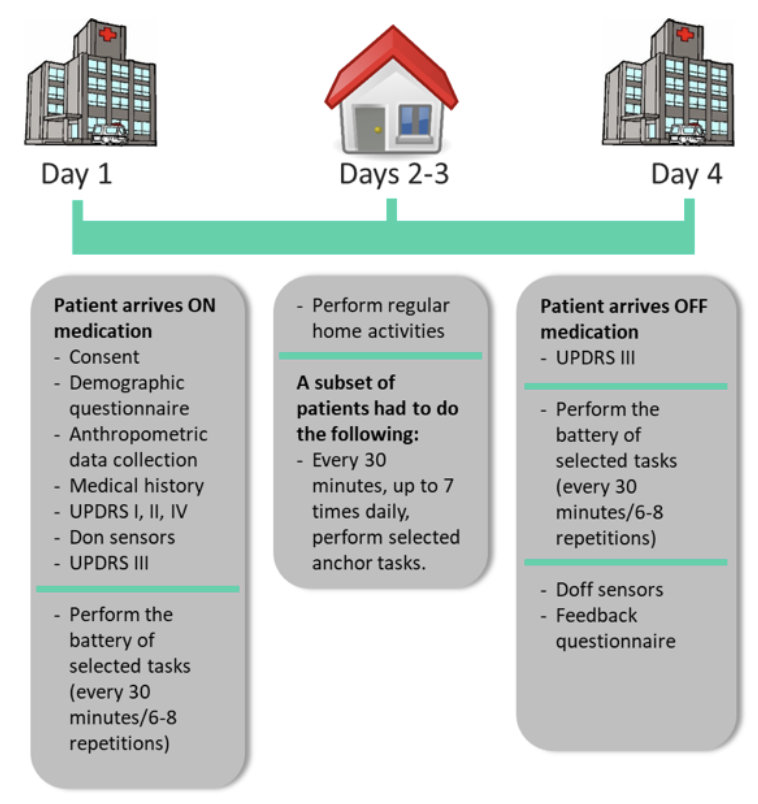
\includegraphics[width=9cm]{report/pics/Day.png}
    \caption{The process by which the dataset was collected \cite{MJFF}}
    \label{fig:my_label}
\end{figure}

\begin{figure}[htbp]
    \centering
    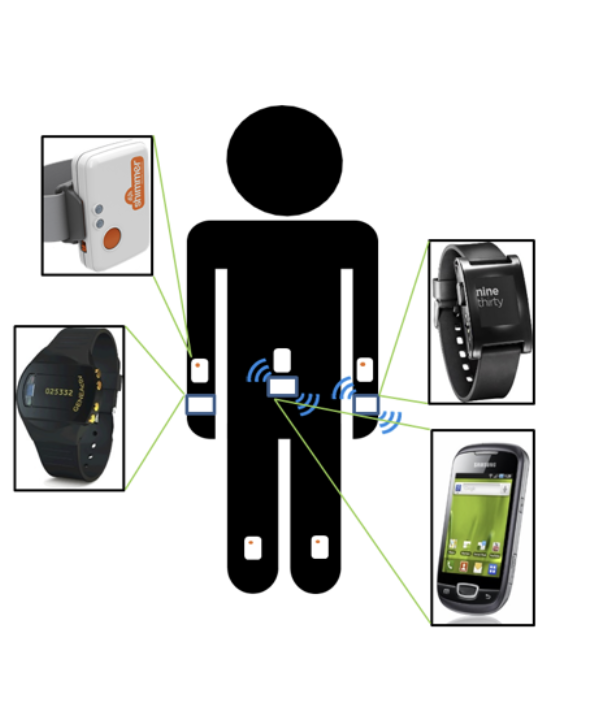
\includegraphics[width=7cm]{report/pics/Sensor.png}
    \caption{About the Sensor Wearing Figure, the Shimmer Sensor is worn on five different parts of the body. \cite{MJFF}}
    \label{fig:my_label}
\end{figure}



A total of 19 subjects, each subject was collected four days of sensor data. On the first day, they had several motor tasks, including standing, walking in a straight line for the 30s, walking in a straight line for 30s while counting backward, walking up and downstairs, walking through a narrow corridor, finger to nose for 15s (twice per arm), regarding other activities: alternating hand movements for 15s (twice for each arm), drawing, typing on the keyboard for the 30s, opening and pouring bottles (three times), arranging pieces of paper in a folder (twice), assembling nuts and bolts for 30s, folding a towel three times and then sitting. On the second and third day, the test subjects wear the sensors at home and record their usual activities and motor tasks, and finally, on the fourth day, the subjects perform the activities from the first day. For this dataset, we will use Shimmer sensor data and datasets to assess the severity of symptoms of Parkinson's disease. Shimmer sensor data is collected in 3 dimensions, per site $(x, y, z)$, with a total of 5 Shimmer sensors corresponding to 15 different datasets being collected simultaneously. The Shimmer sensor (IMU Sensor) collects IMU data as a variable over four consecutive days. The sensor also records data on the abnormal activity of the test subject's Parkinson's disease over the four days. The accelerations in the X, Y, and Z axes collected by the sensor allow us to determine abnormal activity in Parkinson's patients. For example, when a Parkinson's patient has hand tremors, the sensor worn on the hand can record accelerations that are not consistent with regular activity. The dataset also includes ratings for Parkinson's disease (Bradykinesia, dyskinesia, tremor), each with a 0-4, 0 is no symptom occurrence, and 4 is the most severe occurrence of the symptom. So the IMU data collected for abnormal Parkinson's activity can correspond to the rating for each condition. \cite{MJFF}
\\



\begin{figure}[htbp]
    \centering
    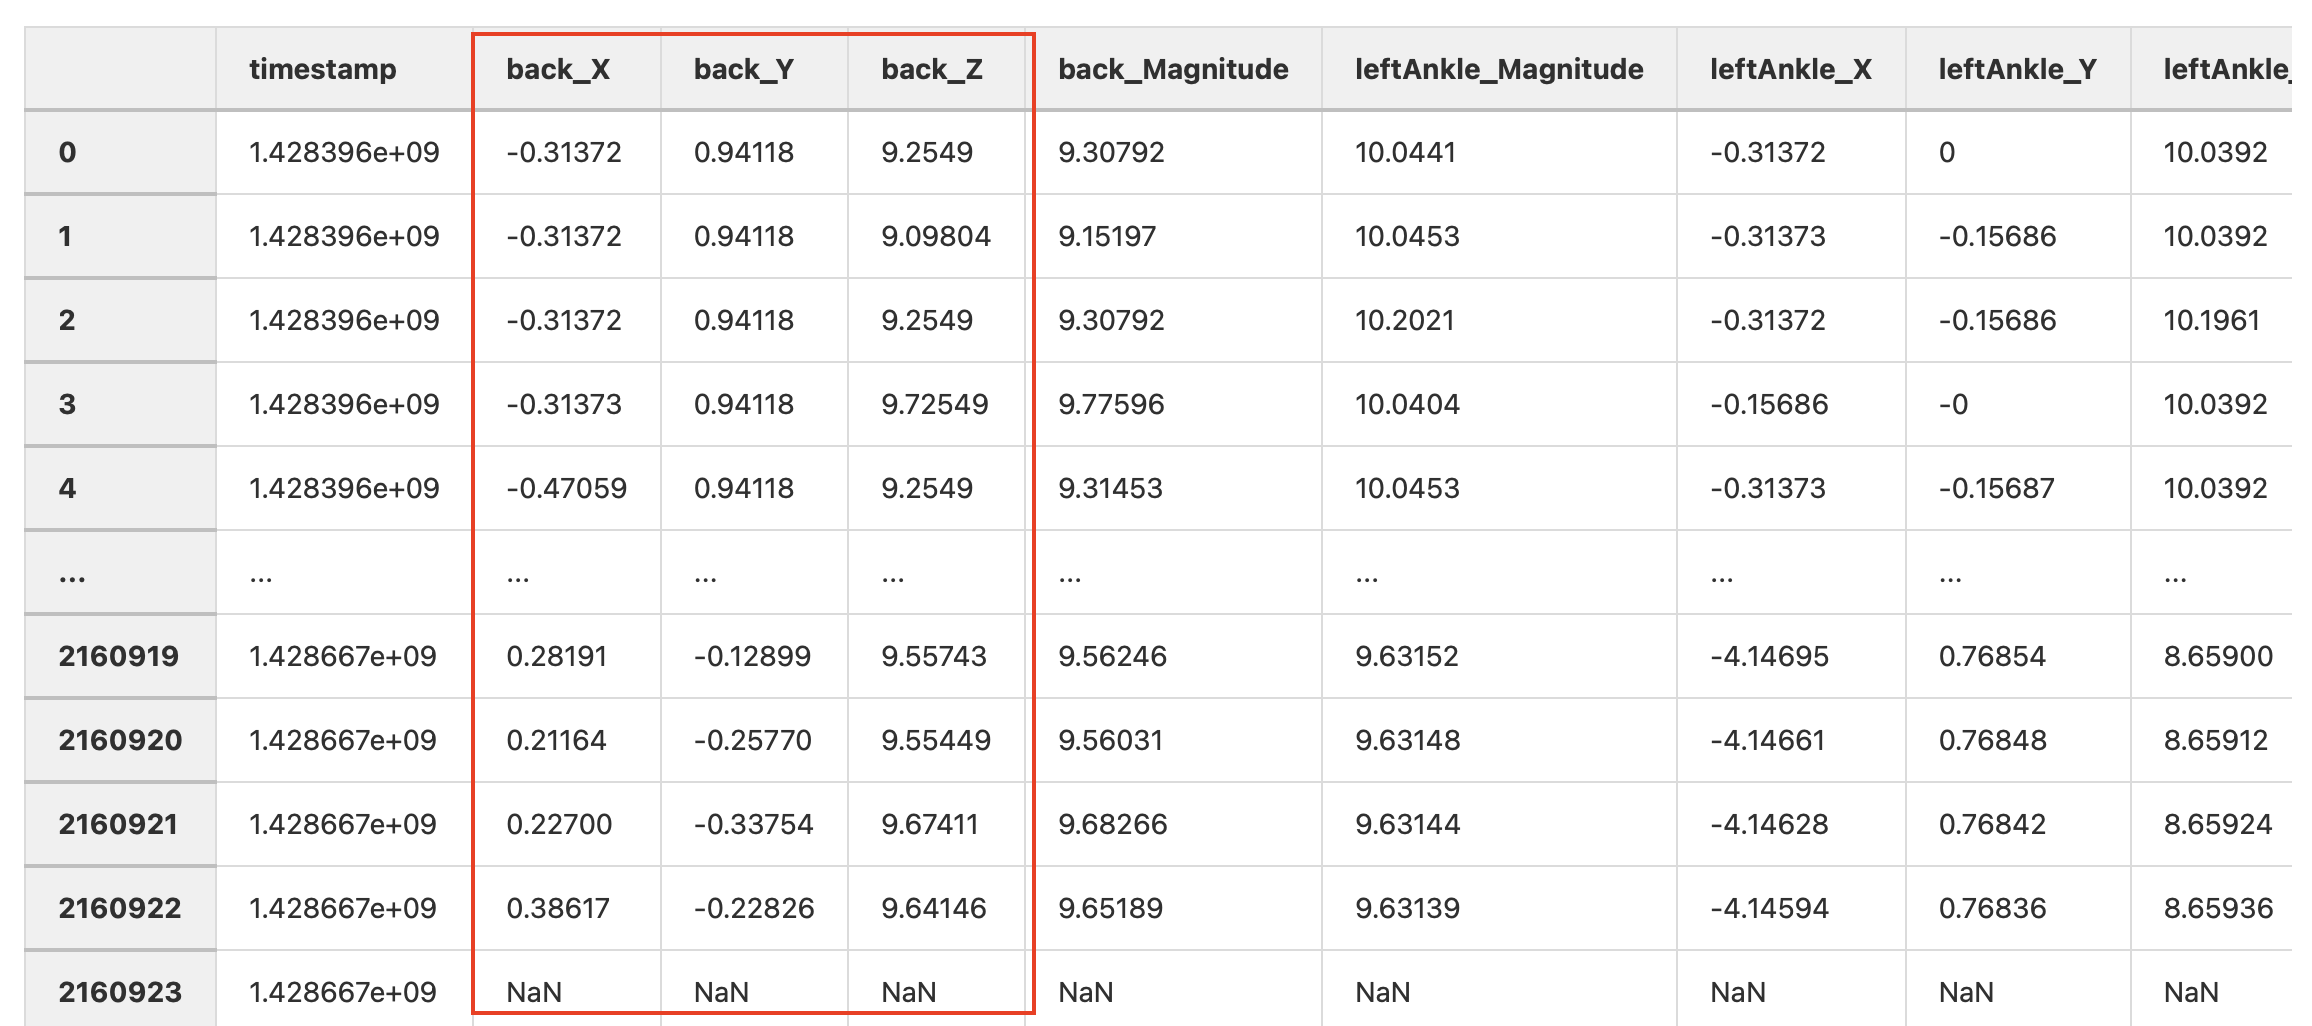
\includegraphics[width=13cm]{report/pics/X.png}
     \caption{IMU acceleration collected from Shimmer sensors worn by Parkinson's patients \cite{MJFF}}
    \label{fig:my_label}
\end{figure}


\begin{figure}[htbp]
    \centering
    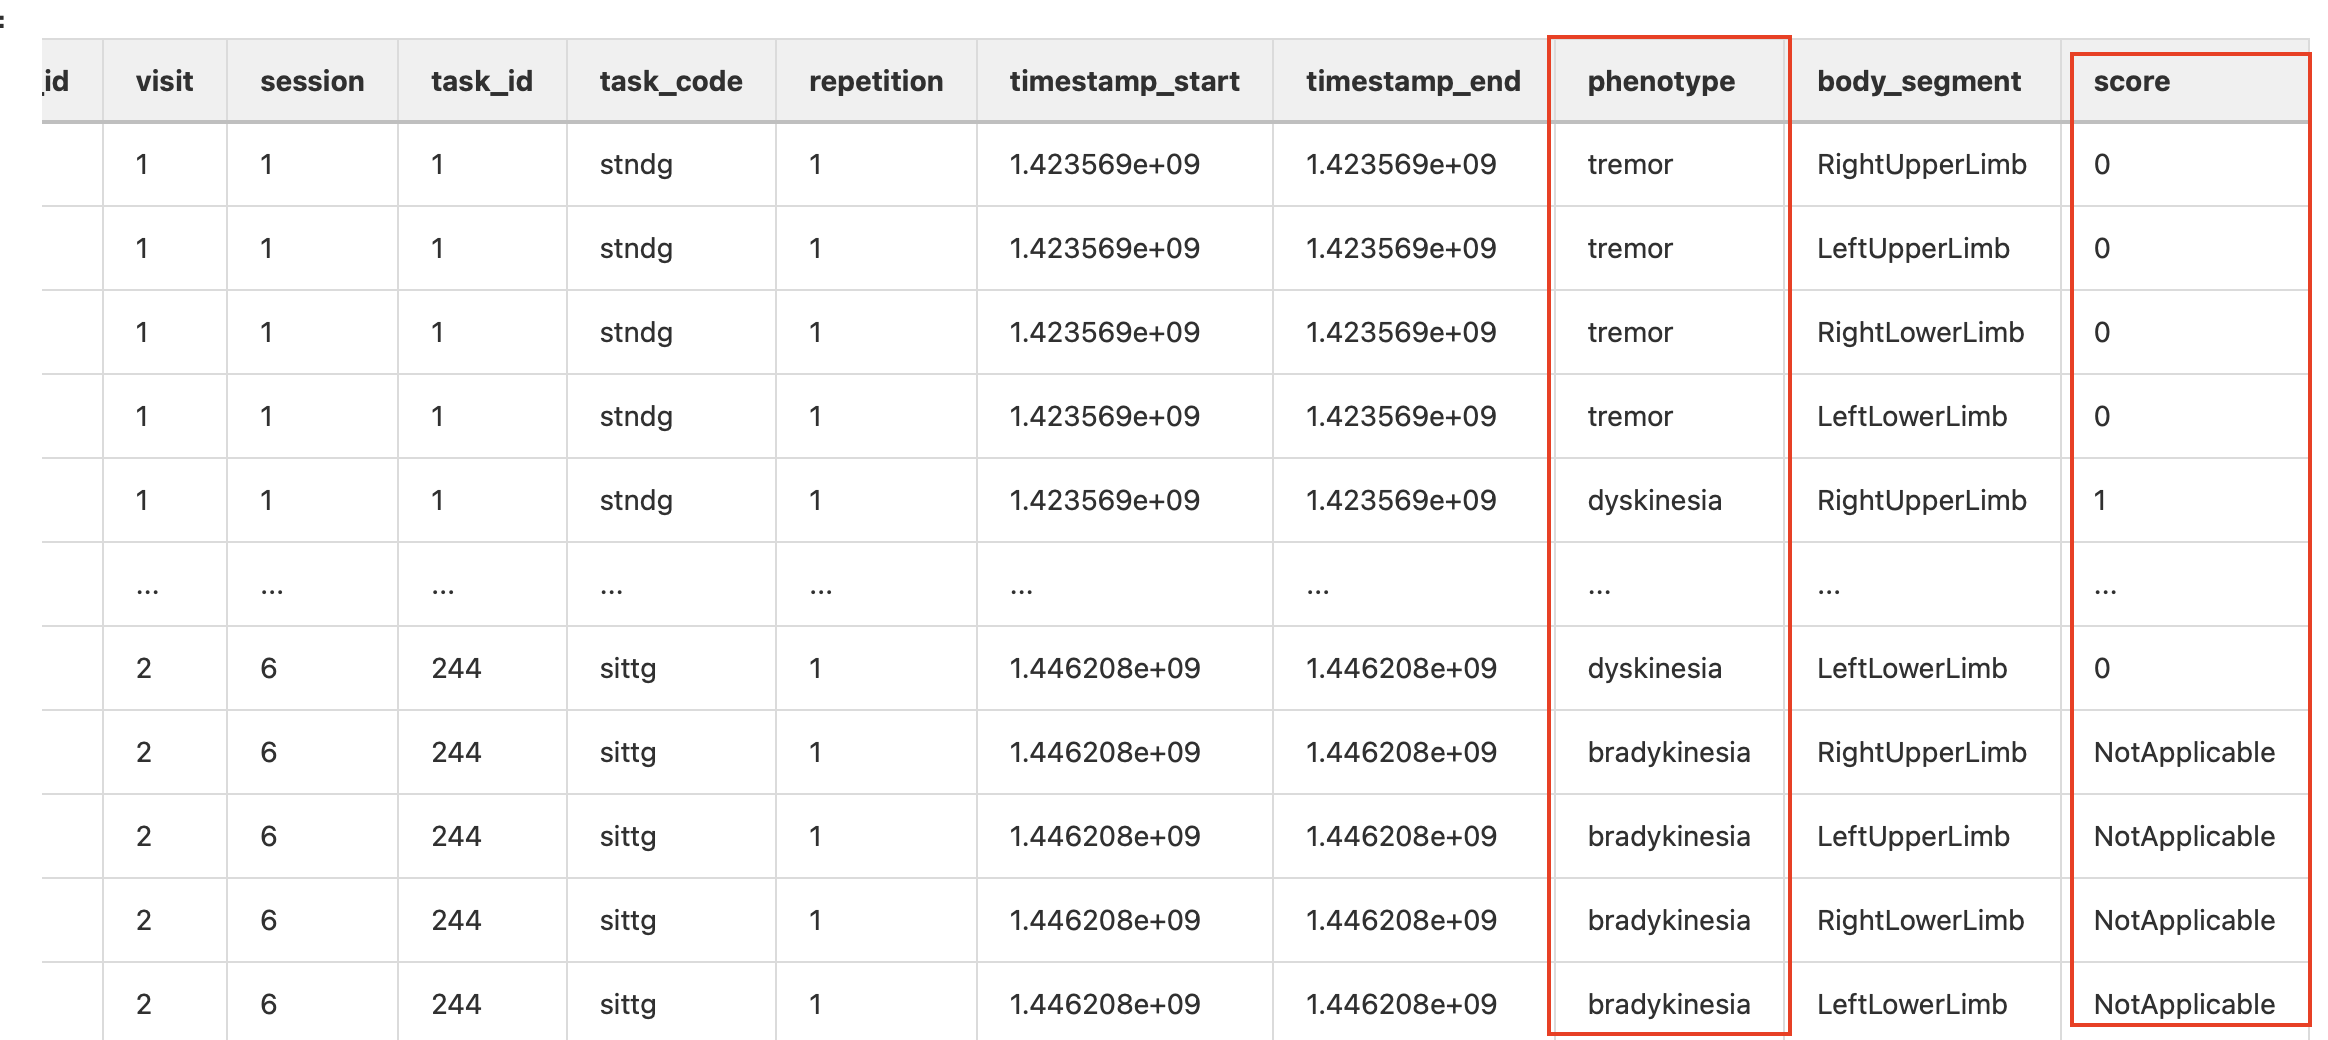
\includegraphics[width=13cm]{report/pics/Y.png}
    \caption{The dataset is rated for Parkinson's disease, with each phenotype corresponding to a score. There will also be some non-applicable data. \cite{MJFF}}
    \label{fig:my_label}
\end{figure}











\subsection{Visualization Analysis}
When visualized, the IMU data helps us understand the data better. Figure 5.5 demonstrates that five different sensors recorded acceleration during dyskinesia, which lasted 32.98 seconds.
\begin{figure}[htbp]
    \centering
    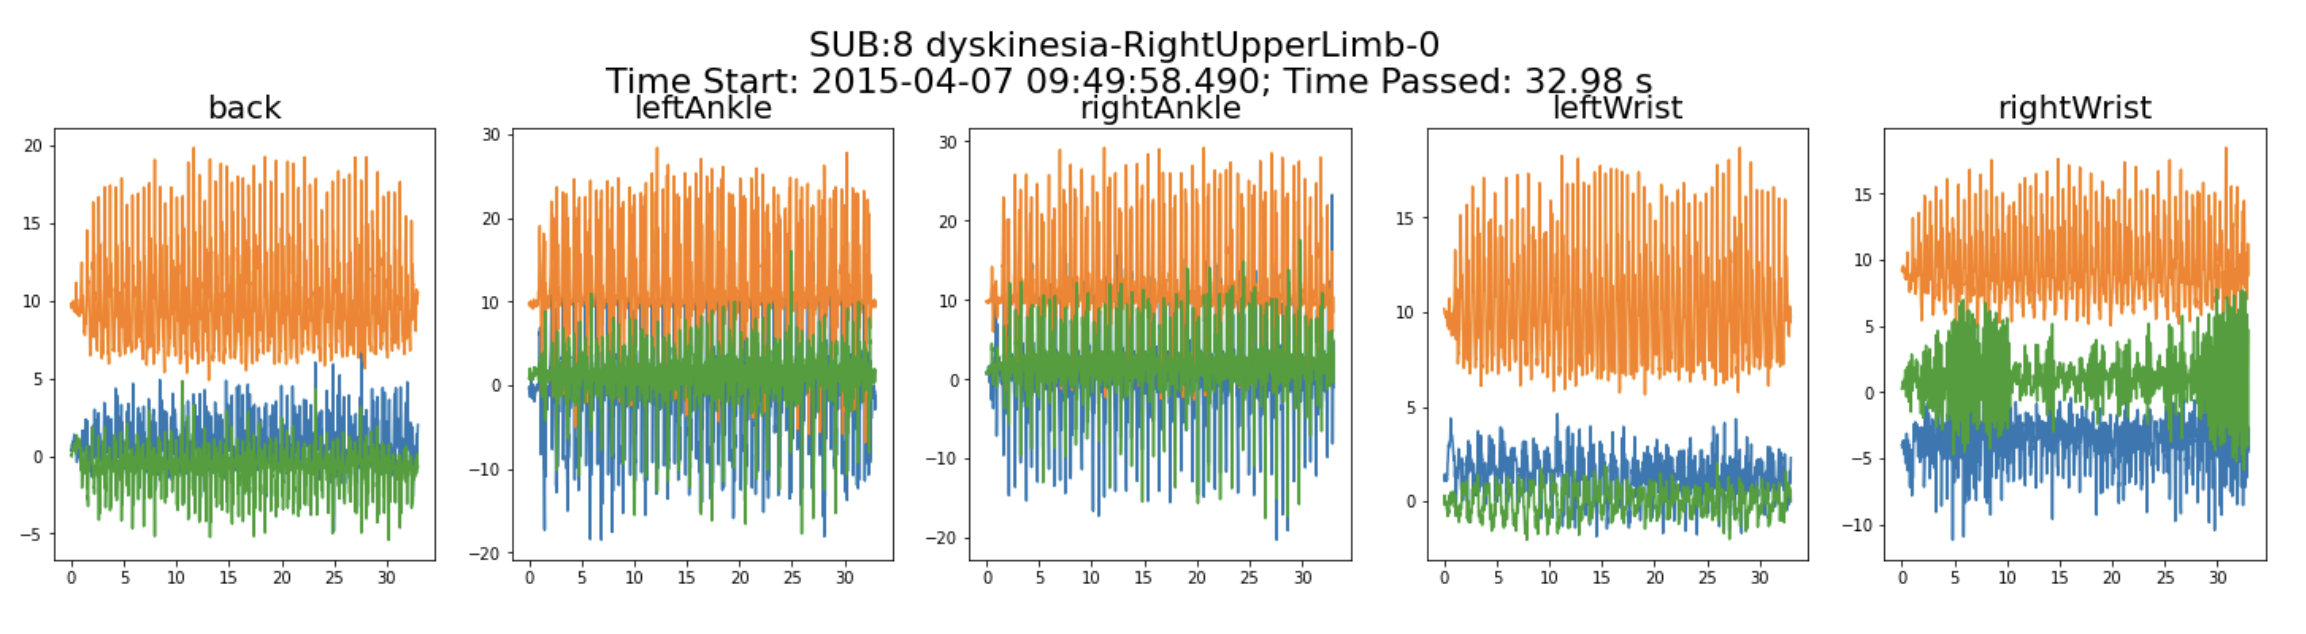
\includegraphics[width=13cm]{report/pics/dyskinesia-RightUpperLimb.png}
    \caption{Acceleration collected by 5 Shimmer sensors in 32.98 seconds accompanied by dyskinesia \cite{MJFF}}
    \label{fig:my_label}
\end{figure}\\

Figure 5.6 shows the percentage of scores for the tremor condition in 34 hours, 52 minutes, and 17 seconds, and we can see that 0 scores account for 72.75\% of the scores. The scores of dyskinesia and bradykinesia are also shown. In bradykinesia, the percentage of "none" and "yes" is significant. Therefore, it cannot be used for motor retardation disorders when quantifying information loss. There is also the proportion of simultaneously rated bradykinesia, again with "0" occupying most of the time and rating "4" occupying very little of the time. Most of the time, patients with Parkinson's disease are 'on' state, so the severity of Parkinson's impairment is 0. The ratings '1-4', on the other hand, indicate the severity of Parkinson's impairment from mild to severe.

\begin{figure}[htbp]
    \centering
    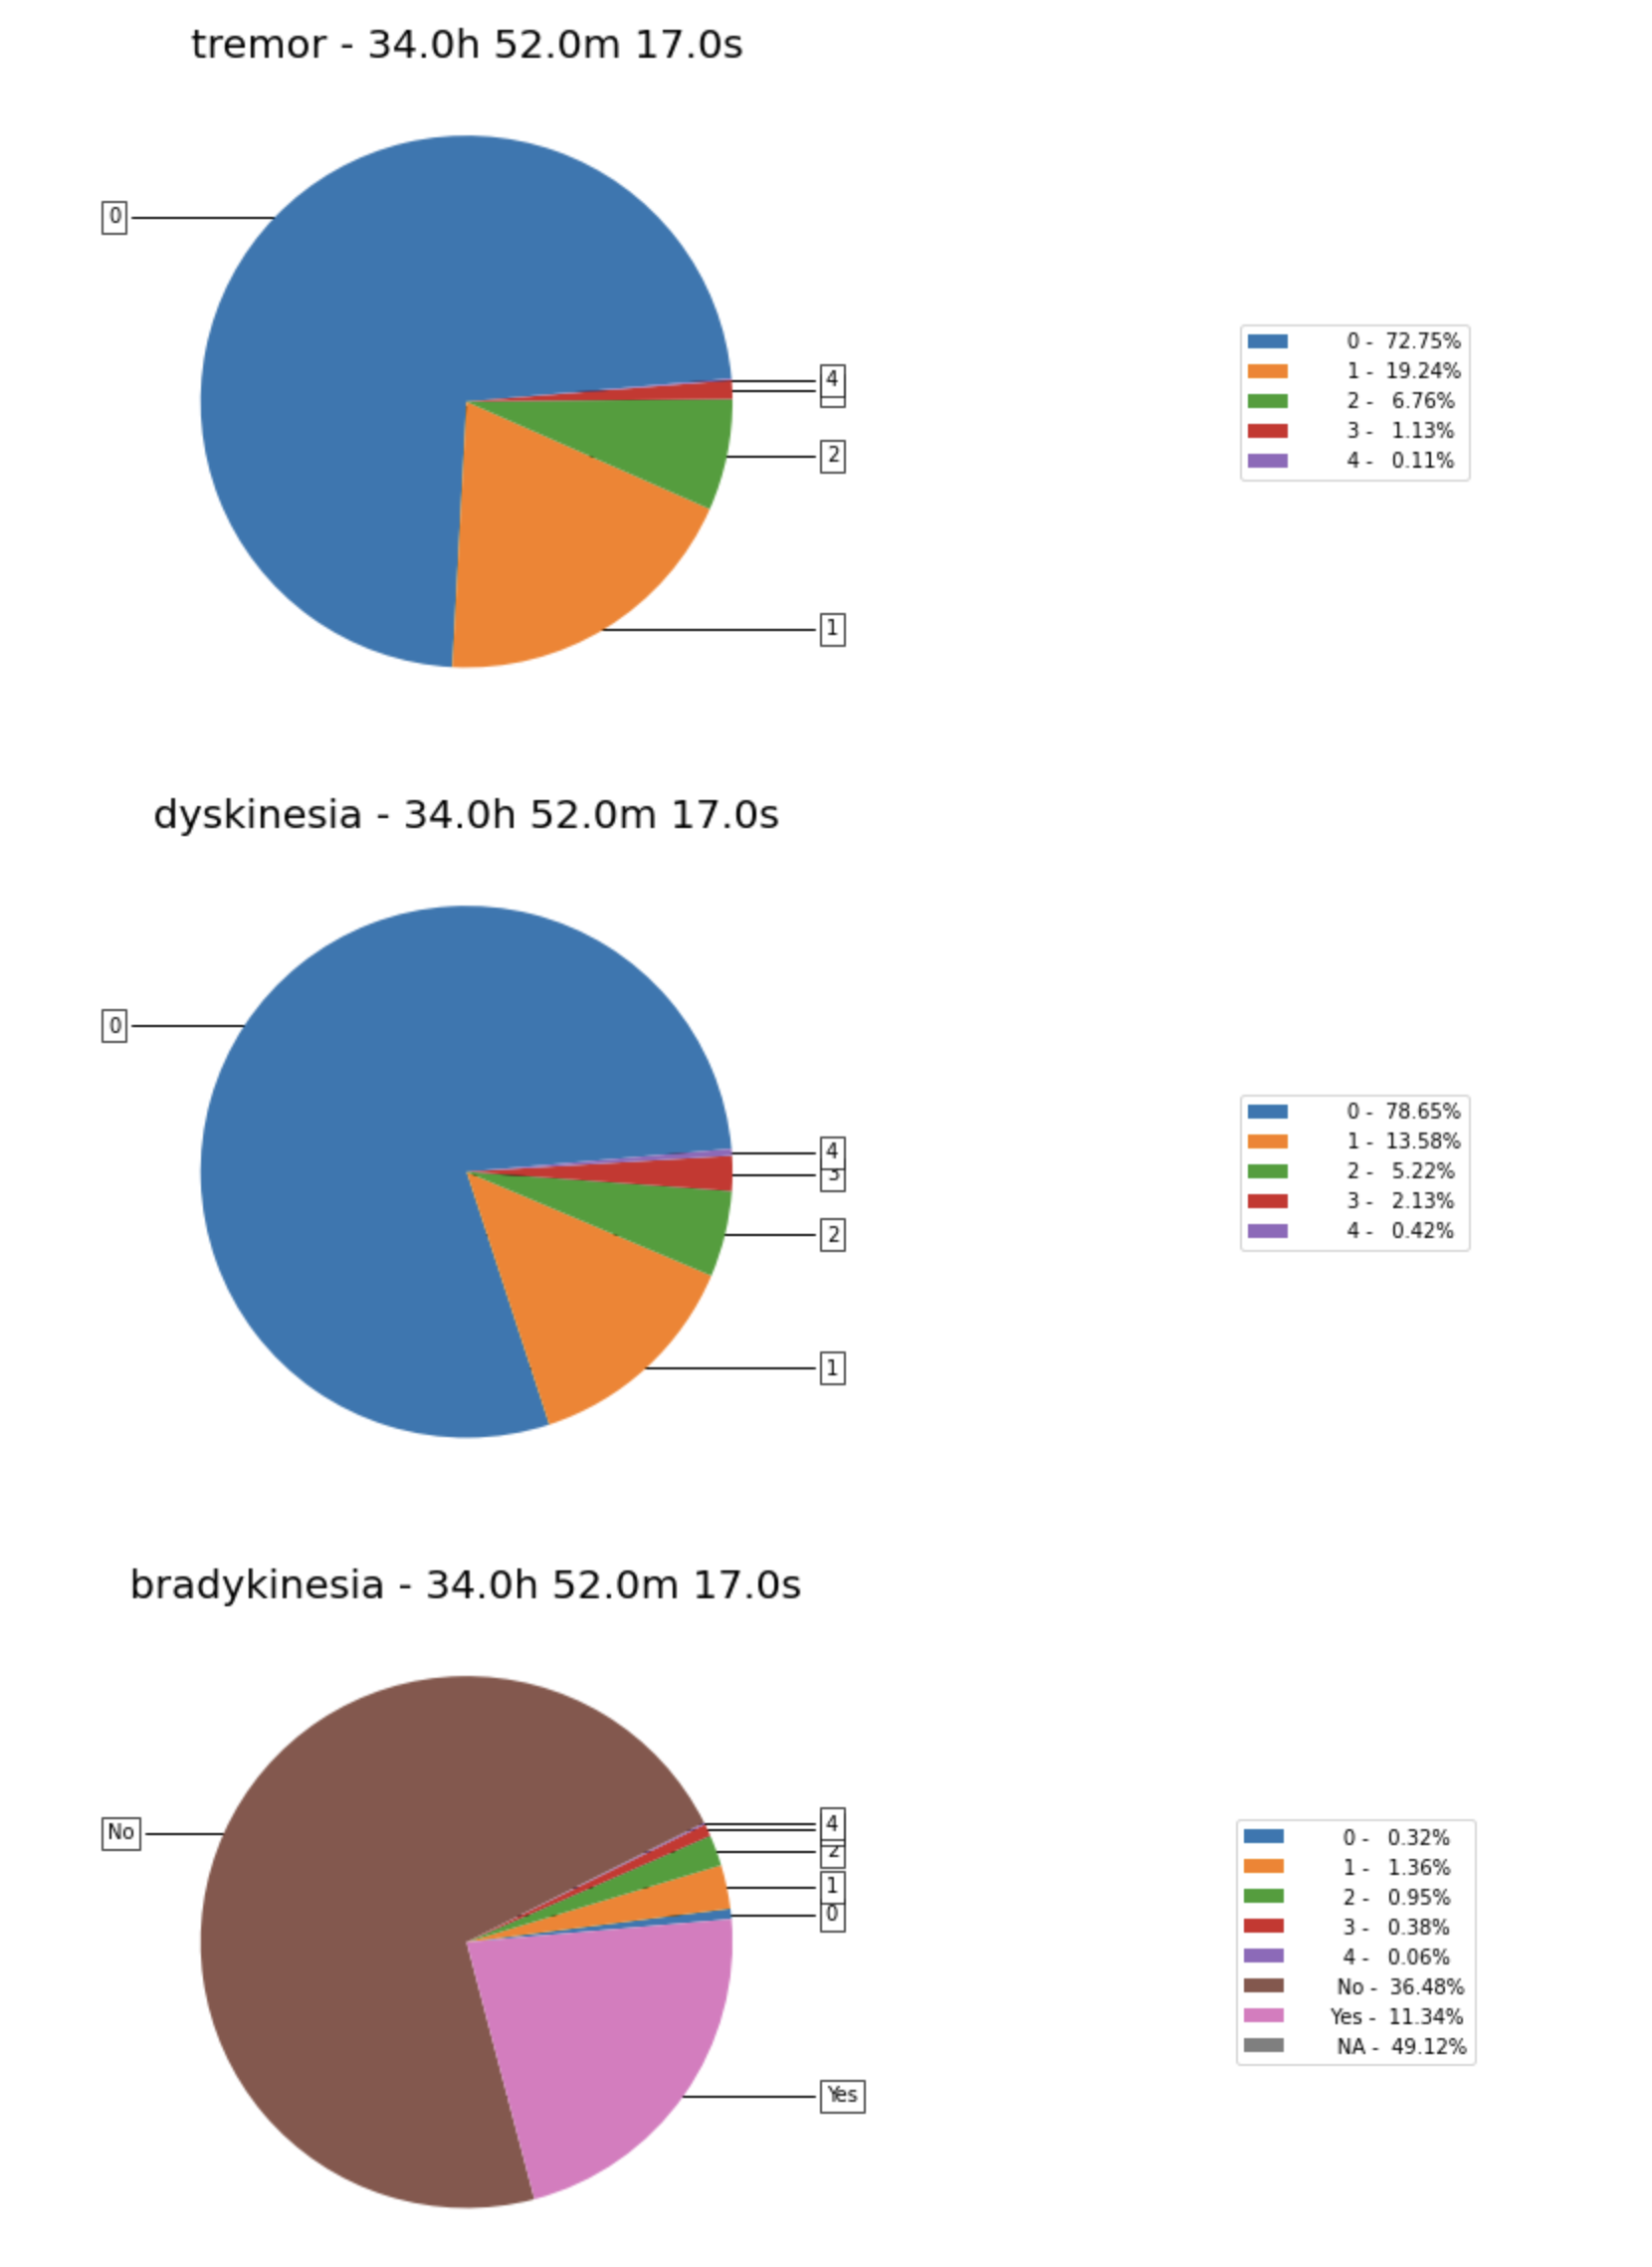
\includegraphics[width=12cm]{report/pics/PD.png}
    \caption{Diagram showing the ratings of the three Parkinson's conditions at the same time. \cite{MJFF}}
    \label{fig:my_label}
\end{figure}\\

\\ \hspace*{\fill} \\
By visualizing the observed dataset, we first want to associate the IMU data collected by the Shimmer sensor with the Parkinson's disease symptom scores via timestamp mapping, i.e., create a new dataset that includes both IMU data and symptom scores. However, if we use timestamped 1Hz sampling to match the data, there is a significant loss of information. Because the IMU sensor has a sampling rate of 0.02s (50Hz), we map the symptom score scores without changing the sampling rate. From Figure 5.4, we can see the start timestamp and the end timestamp for each Parkinson's disease condition, and this period is typically 30-34 seconds. Theoretically, we have 50 sets of IMU data corresponding to 1Hz, so 30s to 34s corresponds to 1500-1700 points. We have 5 Shimmer sensors corresponding to 3 dimensions of $(x, y, z)$ acceleration data, which means we will get at least 22,500 points under one symptom score. For our 19 patients, each with multiple symptoms, it is challenging to store such a large amount of data. Traversing the patient's data is also tricky due to the high performance of the running memory. \\
\\ \hspace*{\fill} \\
To address the operational difficulties caused by a large amount of data, we should consider not storing all the data, not traversing all the patient data, and creating a new dataset. Therefore, we use a new test set, i.e., for each symptom scoring time, we select 5s of data, i.e., 5 seconds within 34 seconds of Parkinson's disease. Theoretically, we will get at least 3750 points to read the data faster and quantify the information loss.

\section{Define X and Y in the quantified information}
We choose the IMU data as X. Each Shimmer sensor collects acceleration data in 3 dimensions, i.e., $(x, y, z)$. The original data is the IMU data sampled at 50 Hz. We initially obtain the shape of $x, y, z$ as $(N,250)$, where $N$ is the number of IMU data and $250$ is the dimensionality. We use root mean square (RMS) to associate the x, y, and z into a new X. RMS is defined as:
\begin{equation}
M = \sqrt{\frac{ {\textstyle \sum_{i=1}^{n}x_{i}^{2}} }{n}} =\sqrt{\frac{x_{1}^{2} + x_{2}^{2}+\cdots x_{n}^{2} }{n} } 
\end{equation}
RMS is applied to our data:
\begin{equation}
acc_{rms}(x,y,z) = \sqrt{\frac{x^{2} }{n_{x}} + \frac{y^{2} }{n_{y}} + \frac{z^{2} }{n_{z}}} 
\end{equation}


We defined the rating data for Parkinson's disease as Y, with each rating representing each category in the classification. The shape of Y is (N,) or (N, 1), where N is the number of points of Y. We need to note that the number N of X and Y should be the same.

\section{Reduced sampling frequency on IMU data}
From the previous subsection, we obtained X with dimension 250. To quantify the information loss after reducing the sampling rate. We will resample the acceleration data distribution of X, i.e., IMU, using 25 Hz, 10 Hz, and 5 Hz to get three new X data. We can see that each frequency corresponds to a time of:
\begin{equation}\nonumber
\begin{aligned}
&50Hz = \quad sampling\quad every\quad 0.02s,  &25Hz =\quad sampling\quad every\quad 0.04s  \\
&10Hz = \quad sampling\quad every\quad0.1s,   &5Hz =\quad sampling\quad every\quad 0.2s \\
\end{aligned}
\end{equation}
\\ \hspace*{\fill} \\
The IMU-Shimmer sensor collected our original data set at 0.02s, so we see a data set with an interval of 0.02s per bar. If we resample the data once at an interval, we are resampling at 25 Hz, and the new data is 0.04s per interval, and so on. Although we resample the data, the data points in our X and Y data sets are the same, and each point's dimension changes.


We can see that the X shape obtained after resampling with reduced sampling frequency is
\begin{equation}\nonumber
\begin{aligned}
X_{50Hz}:(N,250) \to  X_{25Hz}: (N,125) \to X_{10Hz}:(N,50) \to X_{5Hz}:(N,25) 
\end{aligned}
\end{equation}








\chapter{Quantifying information loss based on K-nearest neighbor (KNN) classification algorithm}


\section{K-nearest neighbor (KNN) algorithm}
K-Nearest Neighbor (KNN)\cite{peterson2009k} is a commonly used supervised learning method that works by a straightforward classification mechanism by measuring the distance between different feature values. \cite{altman1992introduction} KNN is based on the idea that if the majority of the k most similar (i.e., most adjacent) samples in a sample's feature space belong to a particular class, then that sample also belongs to that class. From the Y we defined in the previous section, we can classify each of the 0-4 symptoms of Parkinson's disease into five different categories. Thus, when we use KNN classification, the data from IMU are classified into different categories.\\
Here is a brief description of the KNN algorithm:   \cite{guo2003knn,zhang2017learning}

\begin{itemize}
    \item [(1)]
    Obtain the distance between the computed and training data. We use the Minkowski distance, which extends the Euclidean distance.The Minkowski distance \cite{singh2013k} is defined as:
    \begin{equation}\nonumber
    \begin{aligned}
    D(X,Y) = (\sum_{i=1}^{n}\left | x_{i} - y_{i}   \right |^{p})^{\frac{1}{p} } \\
    \end{aligned}
    \end{equation}
    between two points $ X = (x_{1},x_{2},\dots ,x_{n} )$ and $ Y = (y_{1},y_{2},\dots ,y_{n})$ 
    \item [(2)] Sorting by distance.
    \item [(3)] Select the K points with the smallest distance.
    \item [(4)] The categories to which the K points belong are compared, and the test sample points are assigned to the category with the highest percentage of the K points according to the principle of minority rule.
    \end{itemize}  
    \section{The choice of k}
    When classifying the problem point, the k in kNN is the nearest neighbors we select. The choice of k-value is critical because: the larger the k-value, the simpler the model, the larger the bias and the smaller the variance (significant training error, small test error), and the easier the underfitting. If K is equal to N, then it takes all the instances, i.e., it takes the most points under a specific classification in the instances, which has no practical significance for prediction. However, the larger the value of k, the simpler the model, the larger the bias and the smaller the variance (more significant the training error and smaller the testing error), and the easier the underfitting. \cite{kozma2008k,steinbach2009knn,landau2011cluster,hall2008choice}
    \\ \hspace*{\fill} \\
    We start with k=1 and use the test to estimate the error rate of the classifier, repeat the process, increasing k by one each time, i.e., adding the nearest neighbor, and then select the k with the minimum error rate. It is also worth noting that the value of k is taken as odd as possible to ensure that a more significant number of categories are generated after calculating the results. A similar situation may arise if an even number is taken, which is not conducive to prediction. \cite{deng2016efficient, steinbach2009knn}
    
    
    \section{Summary on knn algorithm}
  The KNN algorithm is a simple and effective classification algorithm and is very easy to implement. However, for an extensive training data set, it is very time-consuming as it needs to calculate the sample distances with test samples and training data set. However, when the data is large, we can present the data in trees, such as kd-tree and ball-tree, and the ball-tree works better for multiple classifications.\cite{10.1145/361002.361007,Omohundro89fiveballtree} The KNN classification also has drawbacks, with low prediction accuracy for rare categories when the sample is unbalanced. In the case of sample imbalance, we get significant errors when quantifying information loss. Also, using KD trees, a large amount of memory needs to be built up when using the ball count model. So as the sample data increases, the KNN algorithm requires more time and memory.
    
    \\ \hspace*{\fill} \\
   
    \section{Quantifying information loss after classification based on knn}
    We recall the formula for information loss (2.9) and the formula for conditional probability (2.7), we can extend the conditional probability, and we obtain:
    \begin{equation}\nonumber
    \begin{aligned}
    &Loss =H(Y|X') - H(Y|X) \\
    &H(Y|X) = -\sum_{x\in \mathcal{X},y\in \mathcal{Y}}p(x,y)\log_{}{p(y|x)} = E_{p(x,y)}\left [ -\log_{2}{p(y|x)}  \right ]   \\
    
    \end{aligned}
    \end{equation}
    
Where $p(y|x)$ can be given to us by the predicted probability after KNN classification, we can find $p(y_{i} |x_{i}) $. Nevertheless, we need to note that we should use the test set of X and Y here to ensure the model's accuracy. After obtaining the probabilities $p(y_{i} |x_{i}) $, we will estimate the conditional entropy using the Monte Carlo method.Specifically about the calculation of information loss, as described below: \cite{luengo2020survey}
\begin{equation}
\begin{aligned}
\hat{H} (Y|X) &= E_{p(x,y)}\left [ -\log_{x}{p(y|x)}  \right ]  \\
& = - \iint p(x,y)log(y|x)dxdy \\
& \approx \frac{1}{N} \sum_{i=1}^{N}  (-\log_{2}{p(y_{i}|x_{i} )} )
\end{aligned}
\end{equation}
\chapter{Evaluation}

\section{Experimental Results}
In order to avoid the degradation of KNN classification accuracy when the samples are unbalanced, we avoid using data from unbalanced samples in our tests. There is a case where the sample data contains only one category, then the KNN classification is meaningless, and the information loss is 0. After visualizing the data in Section 5, we see that the classification categories under bradykinesia disorders contain 'no,' 'yes,' and 'not applicable. There is a case where the sample data contains only one category, then the KNN classification is meaningless, and the information loss is 0. After visualizing the data in Section 5, we see that the classification categories under bradykinesia disorders contain 'no,' 'yes,' and 'not applicable. We filter the 'Notapplicate' points of bradykinesia and reclassify them, i.e., '0' and 'No' to the new '0' category and '1-4' to a new '1' category. So the classification categories under bradykinesia disorders are '0' and '1'. \\

A common task in machine learning is learning and predicting algorithms from data. \cite{RN3} Therefore, we divide the IMU dataset $X$ and the Parkinson's disease score dataset into a test set and a training set. The training set is used to train the model, and the test set is used to do the final evaluation. \cite{hastie2009elements}. When the model is trained, we cannot know how it will perform. We can use the validation set to see how the model performs on new data. The validation set has two purposes, 1. to evaluate the model and tune out the best k for testing KNN classification, and 2. to tune out the hyperparameters so that the model performs best on the validation set. Finally, we use the test set to compute our probability, $p(y|x)$. \cite{RN4} \\

We selected four patients with Parkinson's disease, i.e., patients 3, 6, 7, and 9. After getting the dataset, we will divide the dataset into a specific ratio. Our division ratio is 0.25; the test set is 0.25 of the dataset, and the training set is 0.75. We use the training set to build the KNN classification model and the test set to predict our probability $p(y|x)$. After getting the predicted probability $p(y|x)$, we bring in equation (6.1) and calculate the conditional entropy for each frequency. Once we have each conditional entropy, we calculate the difference between the conditional entropies at different sampling frequencies, the information loss. \\

First, we calculated the information loss on the left wrist of four patients under three conditions with decreasing sampling frequency. where the classification categories of tremor disorders were, '0', '1', '2', '3'. '4'. Dyskinesia disorders were classified in the categories '0', '1', '2', and bradykinesia disorders are classified in categories '0' and '1' as described above.\\
As in Figure 7.1, the blue, green, and orange lines correspond to the information loss with decreasing sampling frequency for dyskinesia, bradykinesia, and tremor disorders, respectively. We can see that the general trend of information loss is similar. Interestingly, the changes in information loss with decreasing frequency to 25 Hz and 40 Hz are quite close under bradykinesia and tremor disorders. Furthermore, the information loss in dyskinesia disorder has a slightly smaller slope of information loss when the sampling frequency drops to 40 Hz than at 25 Hz. It is noteworthy that the information loss for all three disorders is increased when the sampling frequency decreases from 40 Hz to 45 Hz.\\
\begin{figure}[htbp]
\centering
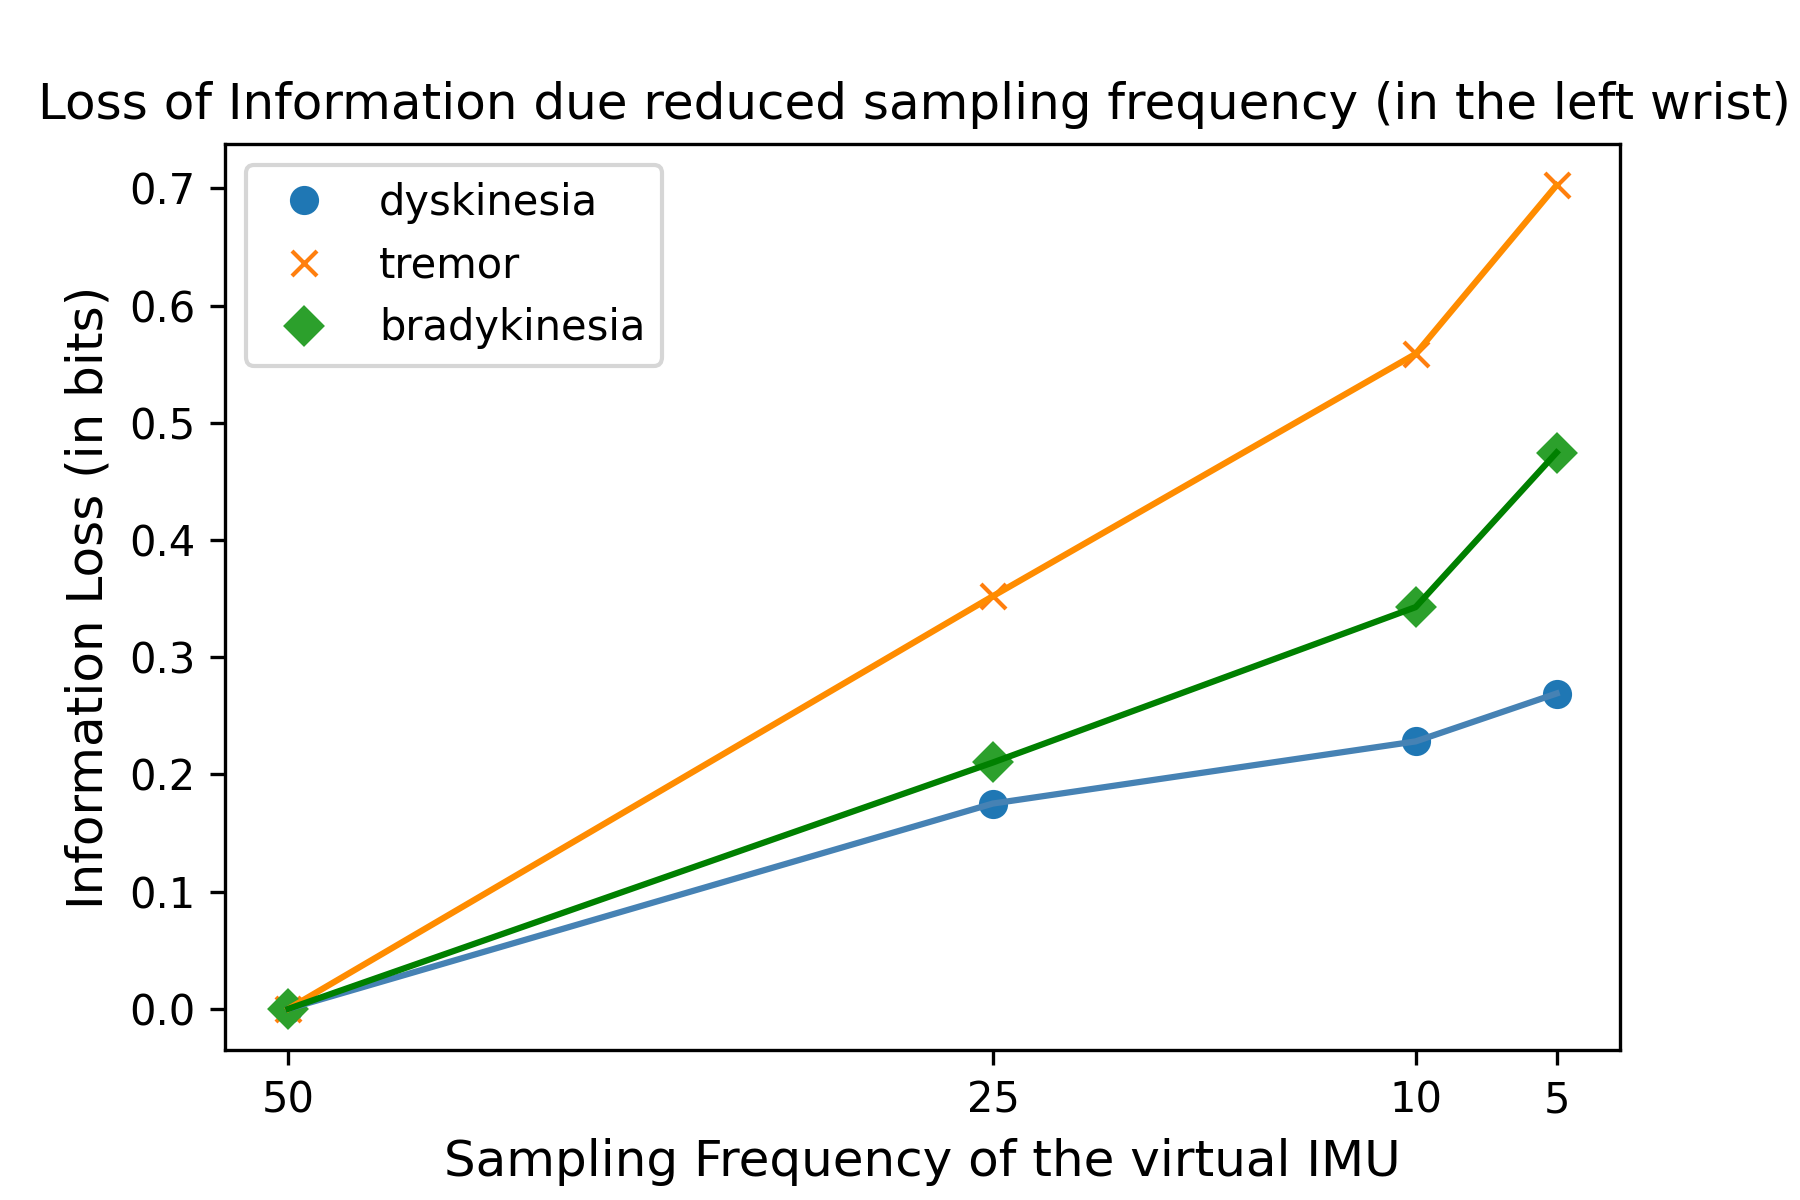
\includegraphics[width=13cm ]{report/pics/7.1.png}
\caption{Variation in information loss with decreasing sampling frequency in patients 3, 6, 7, 9 left wrists under tremor, dyskinesia, and bradykinesia disorders.}
\end{figure} \\

We next proceeded to calculate, for these four patients, the loss of information in the right wrist as the sampling frequency decreased in the three cases. The classification categories for their ratings under the three conditions were the same as for the left wrist.
\begin{figure}[htbp]
\centering
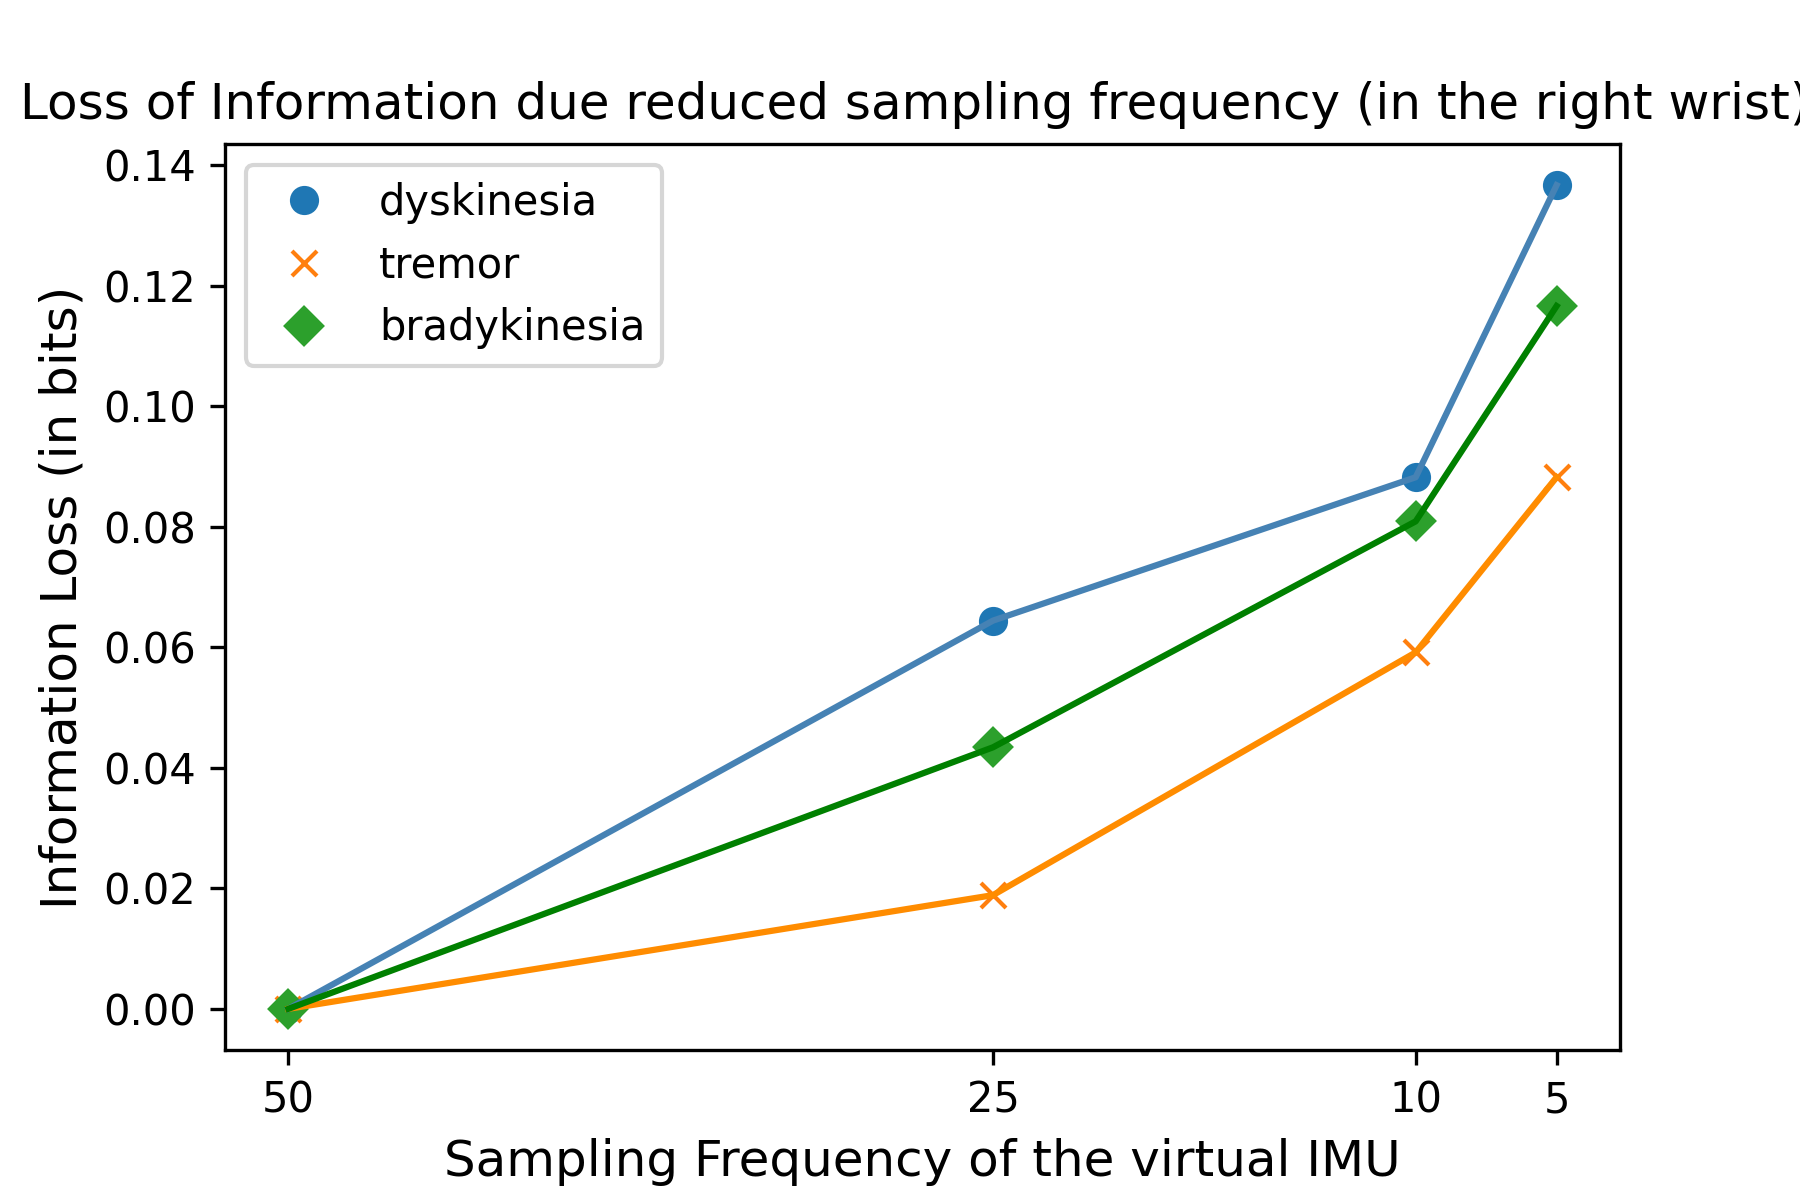
\includegraphics[width=13cm ]{report/pics/7.2.png}
\caption{Variation in information loss with decreasing sampling frequency in patients 3, 6, 7, 9 right wrists under tremor, dyskinesia, and bradykinesia disorders.}
\end{figure}\\
As shown in Figure 7.2, the change in information loss in the patient's right wrist was similar to that in the left wrist in all three conditions, but the information loss in the right wrist was relatively less compared to that in the left wrist.\\

Finally, we calculated the information loss with decreasing sampling frequency for the left ankle of four patients with tremor and dyskinesia. We did not calculate the information loss for bradykinesia because the data sample was unbalanced. There was no "4" in the tremor rating classification, which differs from the left and right wrists.\\
\begin{figure}[htbp]
\centering
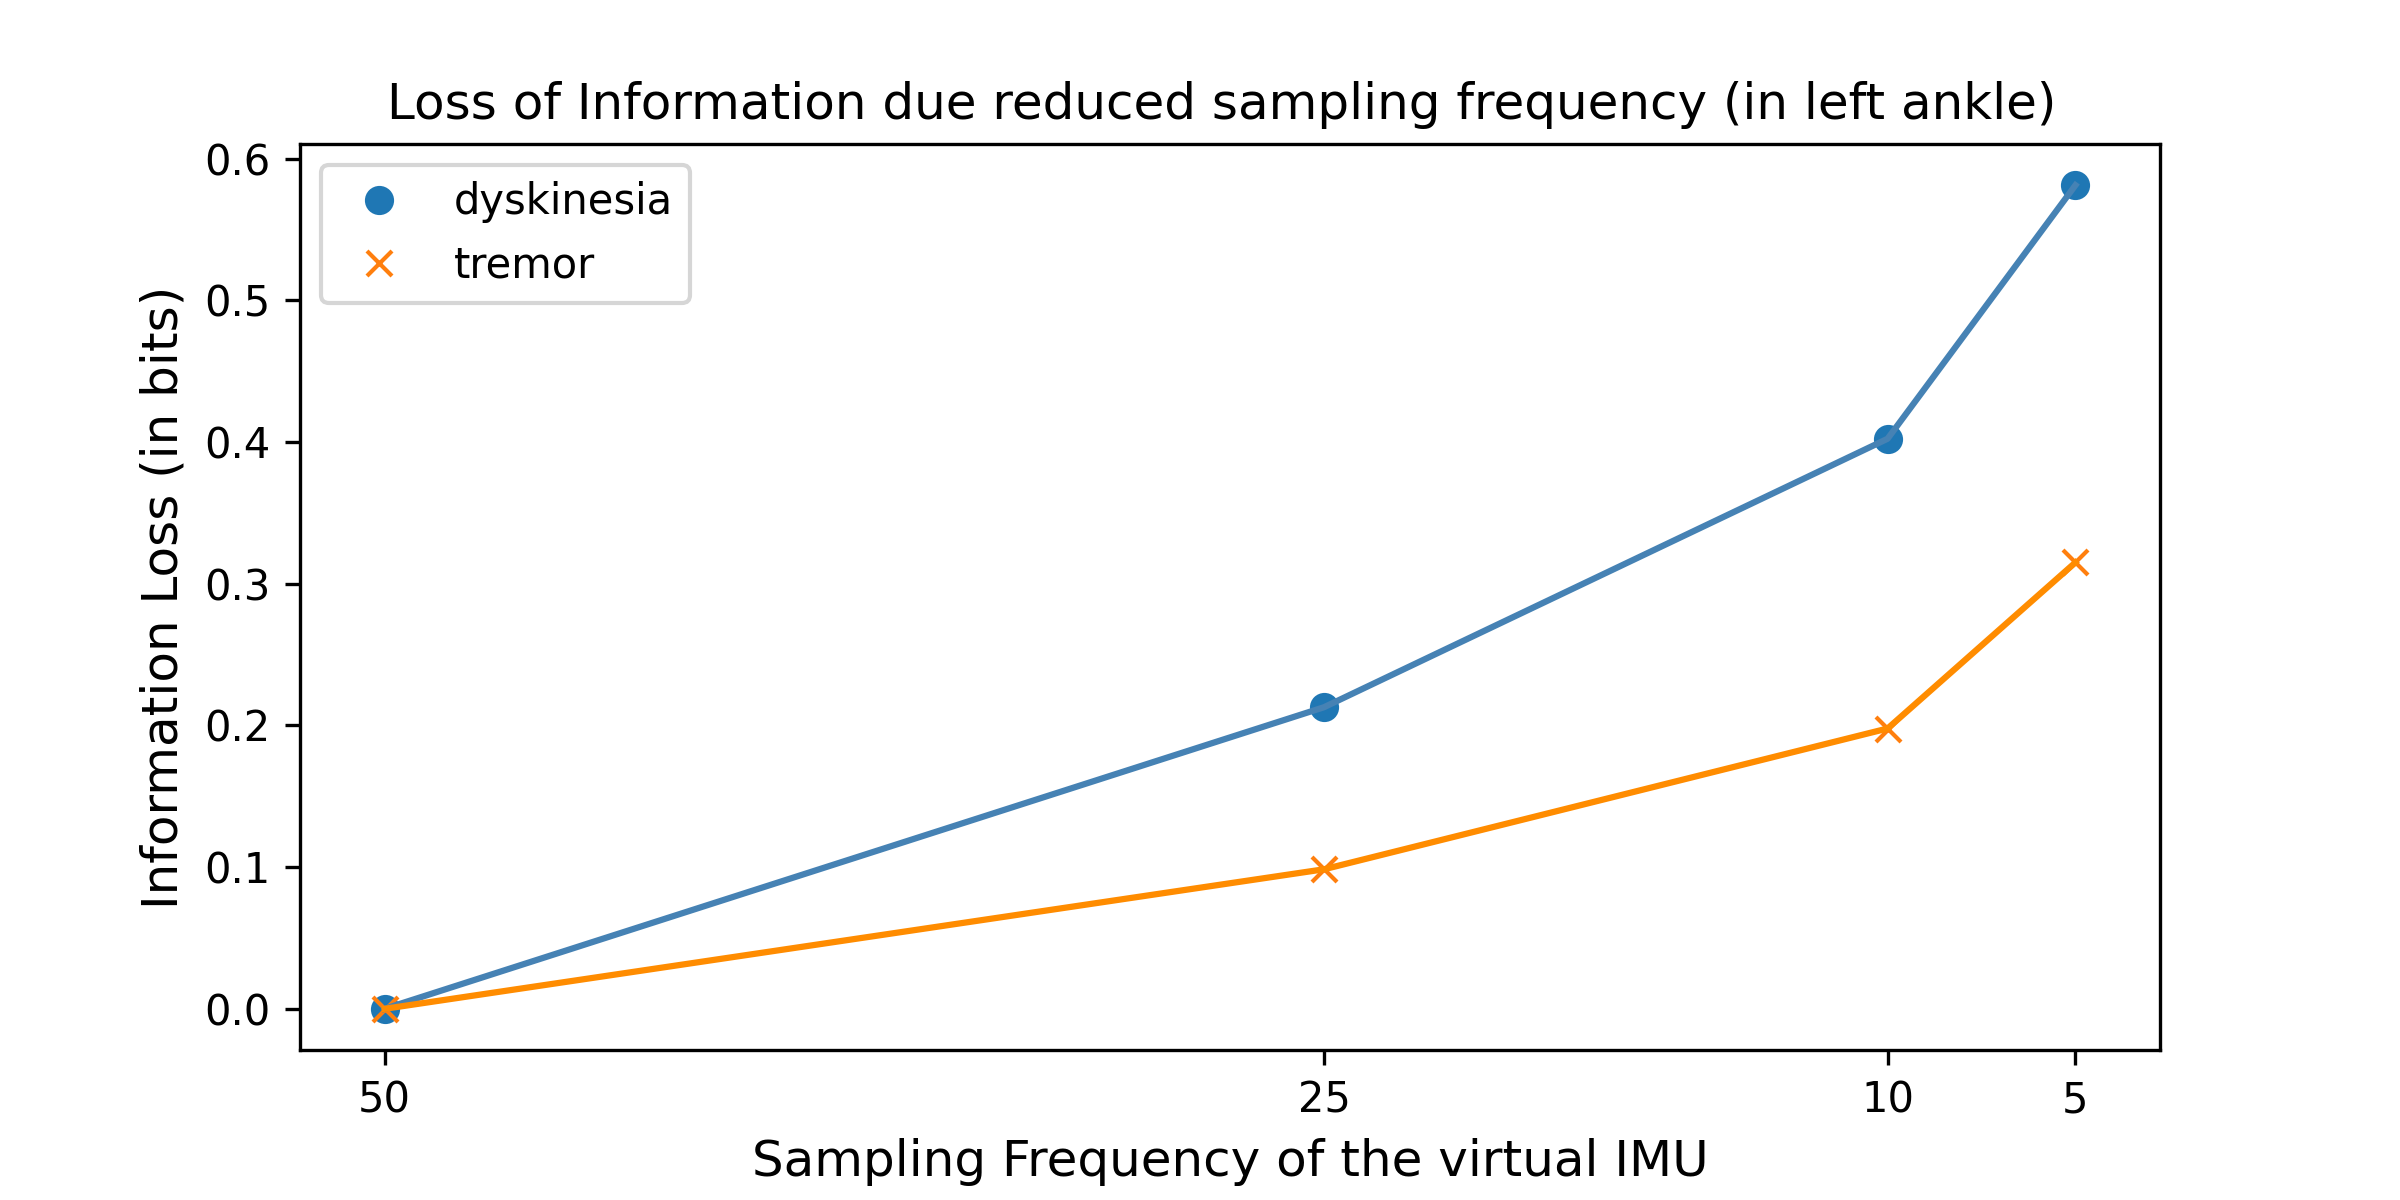
\includegraphics[width=13cm ]{report/pics/7.3.png}
\caption{Variation in information loss with decreasing sampling frequency in patients 3, 6, 7, 9 left ankle under tremor and dyskinesia disorders.}
\end{figure}
As shown in Figure 7.3, the change in information loss is similar for tremor disorders and dyskinesia disorders. However, it is worth noting that the change in information loss for tremor disorder is relatively close when the sampling frequency drops by 25 Hz and 40 Hz. In contrast, the change in information loss for dyskinesia disorder is more pronounced. It is seen that the information loss change is gradually faster in dyskinesia. \\
Combining 7 Fig.1 to 7.3, we can see that the information loss changes under all three disorders are similar at different body parts, with relatively more minor information loss at sampling frequencies down to 25 Hz and some variability at sampling frequencies down to 40 Hz and 45 Hz.


\\ \hspace*{\fill} \\
\section{Results of unbalanced sample data}
In the classification problem with unbalanced data sets, the drawback of KNN is evident, as the minority class is more biased towards the majority class discriminator due to the sample distribution. We can see from the dataset that the severity of Parkinson's disease varies, and typically rating '0' occupies most of the time, while rating '4' does not occupy much time. The sample is unbalanced, increasing our difficulty quantifying the loss of information.\\

\begin{figure}[htbp]
\centering
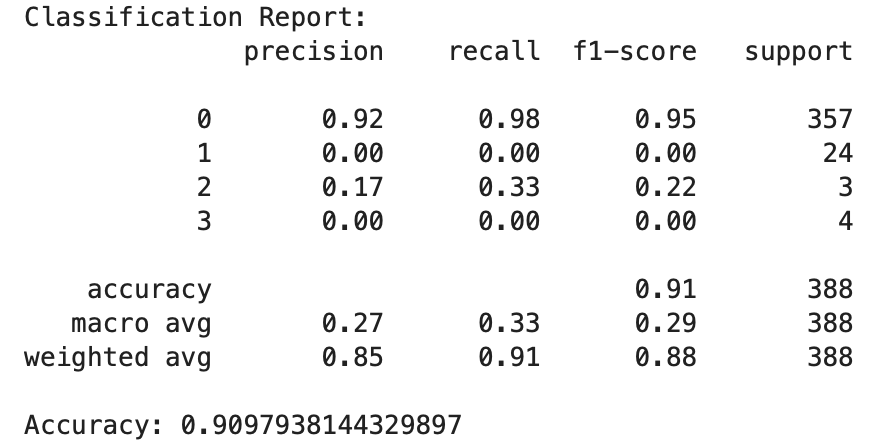
\includegraphics[width=12cm ]{report/chapters/report22.png}
\caption{Patient 9 test set is reported under KNN classification, with different categories corresponding to different data points.}
\end{figure}


\\ \hspace*{\fill} \\
Firstly, we performed KNN classification after classifying the data of patient 9 left wrists under dyskinesia disorder. As shown in Figure 7.4, we have a total of 388 points in our training set, of which class '0': 357 points, class '1': 24 points, class '2' 3 points, and Class '4': 4 points. Such a dataset is unbalanced, and there are far more points in category '0' than in the other categories. kNN classification will incorrectly classify all data points in category 0. Because many categories cannot provide enough training samples, the relatively uniform feature space required by the KNN algorithm cannot be satisfied, making the recognition error larger.\\
We can calculate the information loss when unbalancing the samples and then compare the line plots of information loss. As shown in Figure 7.5, Information loss for patient9 with left wrist dyskinesia disease decreases as the sampling frequency decreases when unbalanced samples are taken.
\begin{figure}[htbp]
\centering
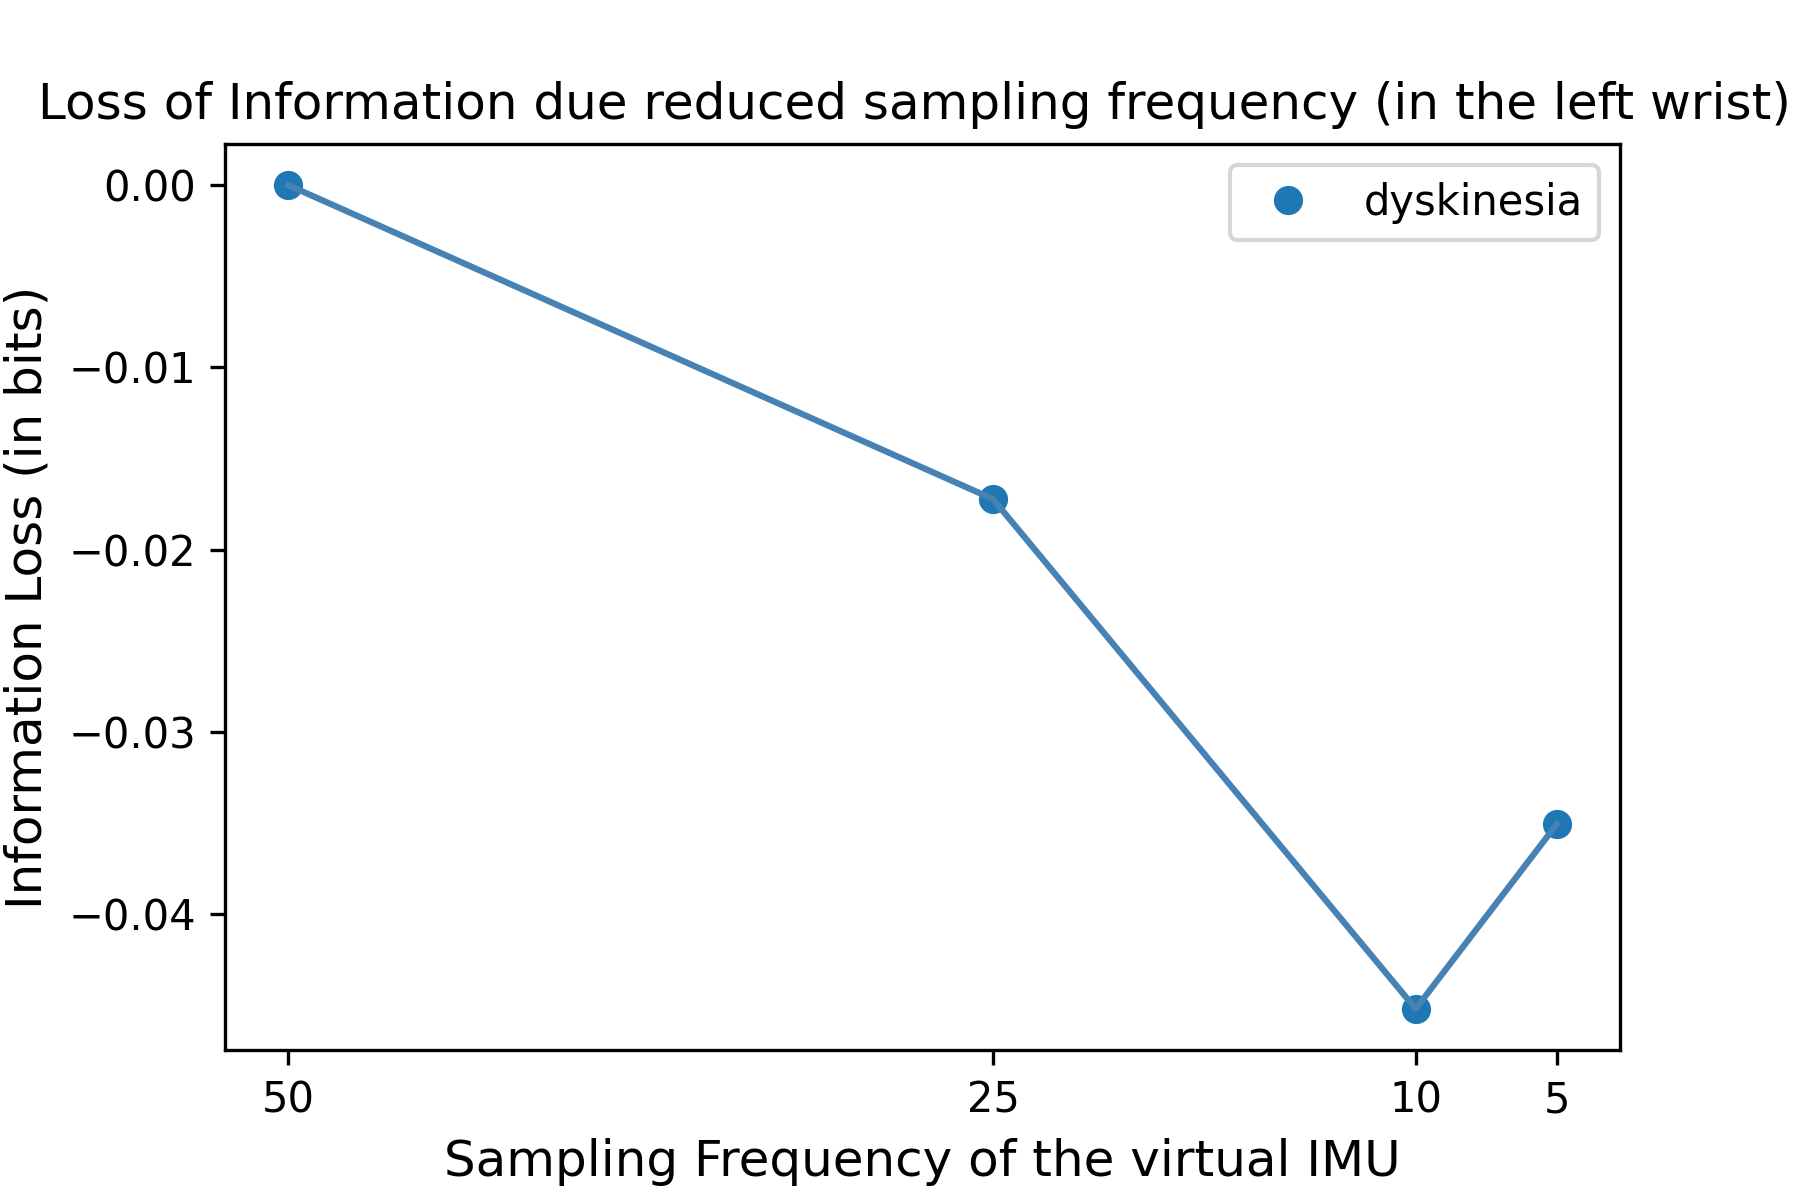
\includegraphics[width=12cm ]{report/pics/dyskinesia_leftwrist9-2.png}
\caption{Information loss with decreasing sampling frequency of IMU sensors in Parkinson's patients9 with left wrist dyskinesia}
\end{figure}\\


As shown in Figure 7.5, we can see a significant error in the information loss and that the information loss is growing inverse. Instead of increasing the information loss, there is a slight decrease; for example, at 25 Hz, there are -0.017 bits of information loss. Such information loss is negligible, and the reason is that most points are classified as '0' during the KNN classification.\\

If our samples are unbalanced, the KNN classification model will learn a priori information about the proportion of samples in the training set. There will be many categories with a focus when predicting with practice. (This may result in better accuracy for the majority category and worse for the minority category.) For example, when the sample size of a category is petite, the probabilities calculated after knn classification are the same as those focused on the majority category, which impacts the calculation of our information loss. To overcome the effect of reducing the sample imbalance KNN classification prediction accuracy, we can weight the categories, for example, use smaller weights for categories with large sample data size. \cite{harrington2012machine} \\
In comparison, we use larger weights for categories with a small sample size. In addition, as the only hyperparameter k of the KNN algorithm, its setting will also significantly impact the algorithm. To reduce the influence of the k value, we can weigh the distance. That is, adding weight to the distance of each point so that the closer points can get a more significant weight. \cite{harrington2012machine}
\\ \hspace*{\fill} \\
Similarly, when calculating the information loss, if there is only one type of classification, the information loss is 0 no matter how to reduce the sampling frequency. Hence, KNN classification is meaningless when there is only one classification category.
\\ \hspace*{\fill} \\
\section{The estimated sampling frequency threshold}
We analyze the calculated information loss results with the differences between categorical categories, Parkinson's disease differences, and where the patient wears the sensor. We could estimate a threshold, the frequency interval where the information loss is minor when the sampling frequency decreases. Our analysis of the information loss plots for the patients showed a similar trend in information loss. When we reduced the sampling frequency to 25 Hz, there was relatively little information loss. However, the information loss increased when we reduced the frequency to 10 Hz and 5 Hz. Comparing the slopes, we conclude that the slopes are relatively small, decreasing in frequency from the original frequency of 50 Hz to 25 Hz. The slope is relatively large, from the original frequency of 50 Hz to the decreasing frequencies of 10 Hz and 5 Hz. therefore, we should choose a frequency between 25 Hz and 50 Hz to obtain a minor information loss at the decreasing frequency. To get a more accurate sampling frequency, we also need to resample the data further and then calculate the information loss. \\
\\ \hspace*{\fill} \\

\chapter{Discussion}
Our aim in these works is to quantify the information loss due to the reduced resolution of IMU sensors in PD symptom classification. As mentioned previously, high-precision sensors tend to be expensive. Therefore, we can consider using lower accuracy sensors, i.e., low-cost sensors in daily life if the information loss is slight due to the decreasing resolution of IMU sensors. Parkinson's patients can use low-cost sensors to monitor activities in daily life without using high-precision medical IMU sensors.
The previous section quantified the information loss when the sampling frequency decreases and derived thresholds for sampling rates from 25 Hz to 50 Hz. Based on KNN classification, we obtained the classification probability, i.e., $p(y_{i} | x_{i})$. We estimated the joint entropy of the IMU dataset and Parkinson's disease by Monte Carlo estimation. We derived the information loss by calculating the difference between the joint entropy. KNN classification, however, has some advantages and disadvantages. \\

\textbf{Advantages of KNN}
\begin{enumerate}
    \item The KNN algorithms are theoretically mature and relatively simple.
    \item Compared with the simple Bayesian algorithm, there are no assumptions on the data, high accuracy, and insensitivity to outliers. \cite{8079967}
    \item  Since the KNN method relies mainly on the limited number of neighboring samples around, rather than on the discriminative class domain approach to determine the class to which they belong. It is more suitable than other methods for classified sample sets with a large number of classes that cross or overlap.
    \item The KNN algorithm is more suitable for automatically classifying class domains with large sample sizes. In contrast, those with small sample sizes are more prone to misclassification using this algorithm.
\end{enumerate}


\textbf{Disadvantages of KNN}
\begin{enumerate}
    \item  Computationally intensive, especially when the number of features is vast.
  \item  When the samples are unbalanced, KNN classification has low prediction accuracy for rare categories.
    \item  KD tree, ball tree, and other models need much memory to build.
\end{enumerate}
Combining the advantages and disadvantages of the KNN algorithm, we should first avoid the situation of data sample imbalance in our quantification process. As shown in the above section, when the data sample is imbalanced, the information loss of quantification is challenging to obtain. However, combined with the actual situation, the initial condition of Parkinson's disease patients, often in terms of severity, is not large, so the imbalance of data samples is difficult to avoid in the classification process. On the other hand, the KNN algorithm is very time-consuming in the case of large amounts of data. Our test dataset was calculated only part of the time for patients with Parkinson's disease. If information loss needs to be computed less time, the KNN algorithm requires more extended time and storage space. So when scaling to large amounts of data, we have to consider the time and storage space issues.
\\ \hspace*{\fill} \\

In addition to this, we need to consider the advantages and disadvantages of the Monte Carlo Method. \cite{earl2008monte,raychaudhuri2008introduction}\\
\textbf{Advantages of the Monte Carlo method}
\begin{enumerate}
    \item  The error of the method is independent of the dimensionality of the problem.
    \item  No discretization is necessary for persistent problems.
    
\end{enumerate}

\textbf{Disadvantages of the Monte Carlo method}
\begin{enumerate}
    \item The errors are probability errors.
    \item usually requires more computational steps N.
\end{enumerate}
Combining the advantages and disadvantages of the Monte Carlo method, we recall that the shapes of our X and Y are (N; 250, 125, 50, 25) and (N, 1). First of all, our data are high-dimensional, and when using Monte Carlo methods, we can avoid the computational difficulties associated with high-dimensional data. Also, our N-data points are significant in number so that the error can be reduced when using Monte Carlo simulations.\\
\\ \hspace*{\fill} \\
We combine the benefits of KNN's multi-classification and applicability to large samples with Monte Carlo methods, which are not limited to high-dimensional data and do not require discretization of continuous variables. The thresholds derived from our quantification of information loss need to ensure many data points and balance the sample data. For the Parkinson's disease score dataset, if there are categories other than '0-4', the information loss we de-quantified is not applicable. So we need to preprocess the data and clean up the data points if other categories appear in the rating dataset. Alternatively, if fewer categorical categories appear, such as '0' or '1', we can consider using other categorization methods to quantify the information.








%_______________________________________________
%_____Zusammenfassung, Ausblick_________________________________
\chapter{Conclusion}
We quantified the information loss accompanying the resolution drop of IMU sensors in Parkinson's disease classification by calculating the difference in conditional entropy between different resolutions after the KNN classification. We resampled the data at sampling frequencies of 25 Hz, 10 Hz, and 5 Hz to simulate low-resolution IMU sensors, respectively, and the results showed that the information loss was less for the 50 Hz drop to 25 Hz and more significant for the 50 Hz drop to 10 and 5 Hz. However, limited by the drawbacks of the KNN classifier, if our dataset is unbalanced, we can increase the weights and then use KNN classification again. We can continue to use different classifiers to quantify information loss in the future. For example, other classifiers can be used only for two sample classification categories.
On the other hand, the data of Parkinson's disease patients tend to be large, so KNN classification still has advantages when dealing with large amounts of data. The larger the sample size of the Monte Carlo method, the closer the approximation is to the actual value. Similarly, we can continue to investigate the effect of the choice of k parameters on the information loss in KNN classification. In summary, we conclude that IMU sensors as low as 25 Hz have less information loss and can interpret the results of these works as low-resolution IMU sensors that still work well between 25 and 50 Hz. This could be a promising aspect of using low-cost sensors to study Parkinson's disease.







%%%%%%%%%%%%%%%%%%%%%%%%%%%%%%%%%%%%%%%%%%%%%%%%%%%%%%%%%%%%%%%%%
% APPENDIX
\appendix
%_________Appendix__________________________________

% final tutorial remarks
\ifLSRITRtutorial

% LIST OF FIGURES
\cleardoublepage
\phantomsection
\addcontentsline{toc}{chapter}{\listfigurename} 
\listoffigures 	
% ACRONYM & NOTATIONS
% --> see include/gloss.tex
\ifdefined\AddMyGloss
    \AddMyGloss 
\fi
% BIBLIOGRAPHY
\cleardoublepage
\phantomsection
\addcontentsline{toc}{chapter}{Bibliography}
\bibliography{ref.bib}
\bibliographystyle{unsrt}

\cleardoublepage
% LIST OF FIGuRES
\phantomsection
\addcontentsline{toc}{chapter}{\listtablename} 
\listoftables
% LICENSE 
\cleardoublepage
\chapter*{License}
\end{document}